\documentclass{article}
\usepackage[a4paper, total={6in, 10in}]{geometry}
%\setlength{\parskip}{0.01cm plus4mm minus3mm}

\usepackage{multicol}
\usepackage{enumitem}

\usepackage{listings}
\usepackage{xparse}

\usepackage[superscript,biblabel]{cite}
\usepackage{graphicx}
\usepackage{hyperref}
\usepackage{caption}

\usepackage{blindtext}
\usepackage{dirtree}

\usepackage{xcolor}
\colorlet{cBlue}{blue!80}
\colorlet{cPurple}{blue!40!red}
\colorlet{cRed}{red!60}

\NewDocumentCommand{\codeword}{v}{
    \texttt{\textcolor{cBlue}{#1}}
}

\NewDocumentCommand{\cmd}{v}{
    \textit{\textcolor{cPurple}{#1}}
}

% Styles stolen from https://www.overleaf.com/learn/latex/Code_listing
\definecolor{codegreen}{rgb}{0,0.6,0}
\definecolor{codegray}{rgb}{0.5,0.5,0.5}
\definecolor{codepurple}{rgb}{0.58,0,0.82}
\definecolor{backcolour}{rgb}{0.95,0.95,0.92}

\lstdefinestyle{mystyle}{
    backgroundcolor=\color{backcolour},
    commentstyle=\color{codegreen},
    keywordstyle=\color{magenta},
    numberstyle=\tiny\color{codegray},
    stringstyle=\color{codepurple},
    basicstyle=\ttfamily\footnotesize,
    breakatwhitespace=false,
    breaklines=true,
    captionpos=b,
    keepspaces=true,
    numbers=left,
    numbersep=5pt,
    showspaces=false,
    showstringspaces=false,
    showtabs=false,
    tabsize=2
}

\lstset{style=mystyle}

\title{\Huge Coursework 3: Genshin Impact Simulator}
\author{William Bradford Larcombe \small (K21003008) \\ Pawel Makles \small (K21002534)}
\date{\small Created: 1st March 2021 \\ Last Modified: 2nd March 2021}

\begin{document}
    % Cover Page
    \maketitle
    \begin{figure}[h]
        \centering
        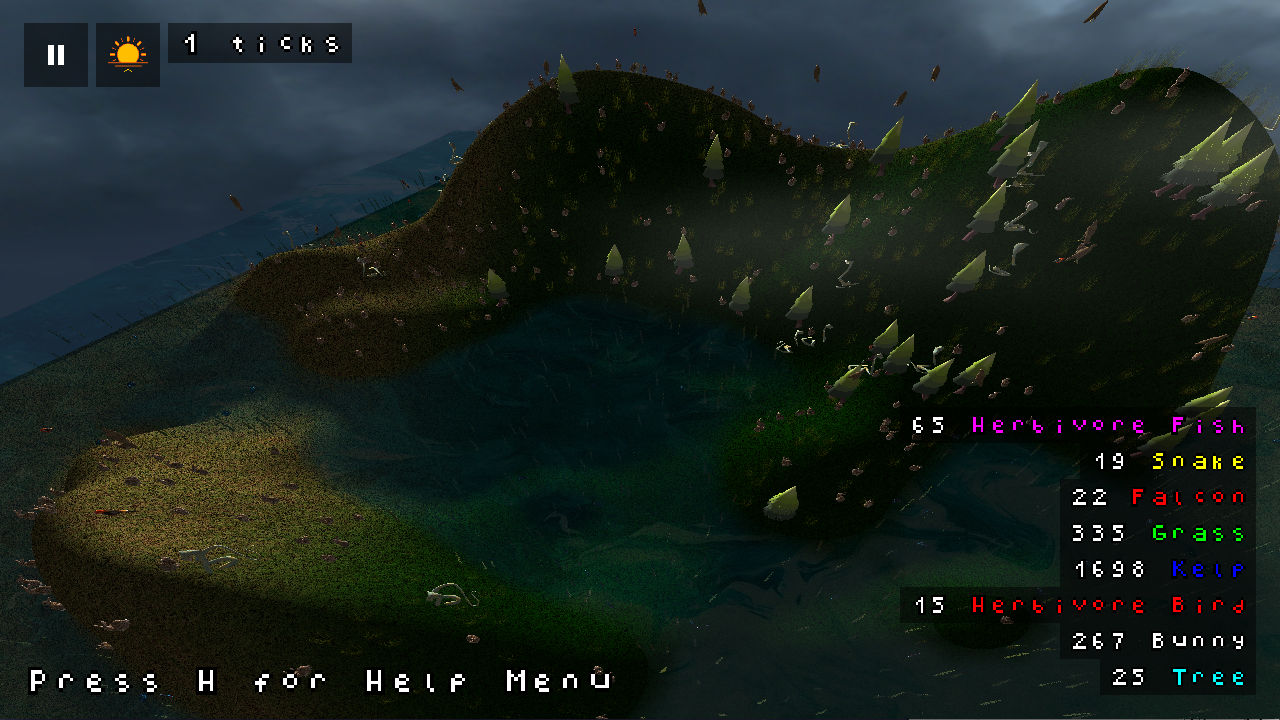
\includegraphics[width=\textwidth]{../screenshot.png}
        \caption{Screenshot of the Simulation}
    \end{figure}
    
    \newpage

    \begin{multicols}{2}
        \section{The Simulation}

        \subsection{Species List}

        \subsection{Species Interactions}
        
        \subsection{Challenge Tasks}

            We completed the following challenge tasks:

            \begin{itemize}
                \item Multi-layered simulation: simulating plants and other foliage as well as aerial animals.
                \item Brain / Behaviour Model: advanced per-entity behaviour.
                \item 3D Rendered Simulation: 3D representation of the simulation world.
            \end{itemize}

        % Layered simulation and interactions between them
        \section{Multi-layered Simulation}
        % this is one of the provided challenge tasks
        We decided that when simulating plants, it would be advantageous to use the same entity system as used for animals to leverage the systems already in place for them. However, it would be necessary for plants and animals to occupy the same space on the simulation grid. 
        
        To allow for this, we created a layered system where different entities could reside on different layers, passing 'over' one another. An Enum was used to define the layers.
        
        After implementing this system for plants, we expanded the system, adding an 'aerial entities' layer. This allowed for birds to fly over other entities without blocking thier movement. A vertical offset was also set for each layer, to allow the aerial layer's entities to be rendered in the air.

        % Could talk about implementation of AI
        \section{Brain / Behaviour Model}

        The AI behaviours of entities are implemented using a system based around 'Behaviours' and 'Brains'.
        
        Behaviours are a basic unit of AI - something like fleeing predators, or hunting prey, or idly wandering around are implemented as behaviours. Behaviours are attached to an entity using the Entity Brain system. The Brain has a list of Behaviours in order of priority. Once per tick, the highest priority Behaviour that reports it can run is run.
        
        The Behaviours and Brains system makes it simple to compose complex AI by attaching simple Behaviours to an entity. This also reduces code duplication, as many entities may need to use the same AI building blocks.

        % Graphics Section
        \section{3D Rendered Simuation}

            One of the first things we did on the project was to bootstrap an OpenGL project and jump straight into 3D, adding an additional dimension to the simulation makes it easier to both see and appreciate the different interactions and behaviours between species.

            \subsection{OpenGL: Nothing to Drawing}

                Typically the setup for an OpenGL context and the subsequent rendering is as follows: configure any native bindings we need (initialise LWJGL \cite{LWJGL}, the library we are using to pull in native bindings), create a new Window and OpenGL context within it, compile required shader programs, upload meshes and textures to the GPU ahead of rendering, and then we drop into a permanent loop which only breaks once the Window requests close or the user initiated some action to close that we caught.

                \subsubsection{Writing and Compiling Shaders}

                    All of the shaders we've had to write are written in GLSL \cite{GLSL}, it is a rather straightforward language used for working with the GPU. Vertices are first processed in the aptly named the ``vertex shader'' where we apply transformation matrices and get everything ready to draw, then the ``fragment shader'' where we figure out how each pixel should be coloured. 

                \subsubsection{Camera and View Projection}

                    For the camera, we decided to just have simple zoom and grab. The eye position is calculated by first finding the distance and height from the point we are looking at.

                    We use $zoom$ to denote the linear zoom factor, $ground$ to denote the angle between the tangent and the water plane, and we use $view$ to denote the angle rotation around the centre point.

                    \[
                        \begin{array}{l}
                            tangent = 5 + 1.1^{zoom} \\
                            distance = tangent \cdot \cos(ground) \\
                            height = tangent \cdot \sin(ground)
                        \end{array}
                    \]

                    Then we find the actual eye position by taking an offset from the position that we are looking at and factoring in the rotation around the centre point.

                    \[
                        \vec{eye} = (x + d cos(view), y + h, z + d sin(view))
                    \]

                    Afterwards, we leverage JOML \cite{JOML} which is a linear algebra library for Java to create a ViewProjection matrix. We specify a perspective of a roughly $ 75^\circ $ field of view with a near plane of $ 0.01 $f, and far plane of $ 1000.0 $f. The camera is positioned at $ \vec{eye} $ and is looking at the centre.

                \subsubsection{Uniforms and the MVP}

                    Given the View Projection matrix, we can multiply it by our Model transformation matrix to find the modelViewProjection, this can be multiplied by the per-vertex coordinates to give the screen-space coordinates for rendering.
                    Matrices are uploaded to the shader through the use of uniforms (memory locations that the shader can access), it is quite straightforward but one key detail we optimise for is that we cache the location of uniform names per-shader in order to be able to skip the look-up every time we render.

                \subsubsection{Lighting the Scene}

                    For this project, we chose to just do simple directional lighting which was used to represent the day-night cycle. The light has 3 properties each of which are exposed and can be modified on the fly during the simulation: Light Direction / Position, Light Ambient and Light Diffuse. We use a subset of the Phong lighting model, (see \autoref{fig:phong}), but chose not to implement specular lighting.
    
                    To get started, we first have to make sure we have all of the data we need from the vertex shader:
                    
                    \begin{lstlisting}
mat4 model;
fragPos = vec3(model *
    vec4(vertexPos, 1.0));
fragNormal = vertexNormal *
    mat3(transpose(inverse(model)));\end{lstlisting}

                    Here we transform the vertex into world-space and also transform the vertex normal, but we run into a minor issue if we were to just use the model projection (see \autoref{fig:normals}), we must use the inverse-transpose matrix to preserve the correct magntiude and retain the correct direction of the normal post-transformation, an article by Lighthouse3D explains the necessity of doing this \cite{lighthouse3d}.

                    Then we can calculate the lighting in the fragment shader, we start off by finding the ambient light on the object, this is pretty simple and we just pass it through:

                    \begin{lstlisting}
vec3 ambient = light.ambient;\end{lstlisting}

                    Next we prepare the light direction and normal vectors for processing, we normalise the normal vector we calculated earlier and then determine the light direction (it could either be an absolute position or relative direction):

                    \begin{lstlisting}
vec3 lightDir;
if (light.dir.w == 0.0) {
    lightDir = normalize(
        light.dir.xyz - fragPos);
} else {
    lightDir = normalize(-light.dir.xyz);
}\end{lstlisting}

                    We can now find the dot product of the normal vector and the light direction, this gives us the strength of the diffuse lighting at that point.

                    \begin{lstlisting}
float diff = max(dot(norm, dir), 0.0);
vec3 diffuse = diff * light.diffuse;\end{lstlisting}

                    Finally, we combine all of the lighting calculations together:

                    \begin{lstlisting}
return objectColour *
    vec4(ambient + diffuse, 1.0);\end{lstlisting}

            \subsection{Uploading and Rendering}
            
                \subsubsection{Mesh to GPU}
            
                    To draw actual objects to the screen, we have to first prepare and upload meshes, we begin by creating a Vertex Array Object \cite{vao} which stores all of the information we provide it ready to render in the future. Each attribute (vertices, normals, UVs, etc) array is given its own Vertex Buffer Object \cite{vbo} to which it is uploaded.
                
                \subsubsection{Textures to GPU}
                
                    OpenGL makes consuming textures very easy, we first load the texture we want using STB Image \cite{stb} which is included in LWJGL, then we configure the texture properties such as alignment and scaling before uploading the buffer we loaded as-is. Some key things to look out for were that textures were always bound to the TEXTURE0 slot since we didn’t need anything more for each mesh, and that OpenGL UV coordinates start from the bottom left which means we flipped all texture resources upside down before loading them. (see \autoref{fig:uvmapping})
            
            \subsection{Optimising Render Pipeline}

                Within our simulation, we quite often have to render hundreds to thousands of objects at a time, so we had to make sure that the simulation could still run on lower-end systems while delivering at least some what of a smooth performance, or at the very least allowed the user to easily look around when the simulation is paused.

                \subsubsection{Face Culling}

                    One of the easiest optimisations to do, although your meshes have to also conform, is to tell the GPU to simply ignore any faces that would not typically be visible. This uses a neat trick by which we order vertices in faces in a clockwise or anti-clockwise manner, so if the GPU detects a specific winding, it can simply reject drawing those faces. In a lot of cases, this should double performance since typically models are quite uniform in how many faces are on each side.

                \subsubsection{Indexing}

                    Indexing is a technique used to create meshes where we generate all of the individual vertex data points and then create an Element Array Buffer which is a list of integers, when drawing triangles we take 3 integers at once which are treated as an index into the attribute arrays that are then used to create the triangle face.

                \subsubsection{Instancing}

                    Another technique to reduce the time on the CPU and let the GPU work in parallel, is to send all the transformation matrices required at once to draw any amount of uniquely positioned meshes. On modern hardware (supporting OpenGL 4.3+), which does not include Mac and Mac M1, we can take advantage of a new extension allowing the use of Shader Storage Buffer Objects \cite{ssbo}. SSBOs allow us to upload a huge amount of data to the shader where it can be consumed as if it were a normal uniform, if the feature is present on the machine \cite{extension-list}, the shader code is modified at runtime to add support for the use of SSBOs. Once enabled, we can instead use glDrawElementsInstanced instead of individually drawing the mesh at each transformation. This has a noticeable effect on devices that support the feature.

                \subsubsection{Mesh Optimisation}

                    One of the biggest bottlenecks on lower-end hardware is just the sheer amount of faces and vertices we want to render, to combat this, we pre-processed all of the meshes we use using Blender by using the Decimate filter (see \autoref{fig:decimate}).

                \subsubsection{Dynamic Level of Detail}

                    Continuing from the previous section: For high level of detail (camera is nearby), we chose to aim for about 1 to 2k faces per object, then halved it for medium and low levels of detail. Before performing a render pass of entities, we first calculate the distance between the camera’s eye position (calculated earlier) and the entity’s current location, then we resolve this to a suitable level of detail such as high, medium, low, or do not render at all.


        % other provided tasks that we haven't done:
        % \subsection{Weather}
        % \subsection{Disease}
        
        \section{World Generation}
        The simulation takes place on a procedurally-generated world. This allows for different starting conditions and therefore different results for each run.
        
        Generation of the world is done in four stages:
        
        \subsection{Biome Generation}
        
        Firstly, a \cite{FastNoiseLite} instance is created, and used to create a randomised biome map. This affects the ground colour and what entities may spawn later on.
        
        \subsection{Heightmap}
        
        A second noise is used to create the heightmap. This creates variation in the vertical level of the ground, creating an interesting terrain with high and low areas. Areas under a certain height level are considered to be underwater; underwater areas have a different ecosystem.
        
        The heightmap is adjusted so that areas outside a circle around the centre of the world are smoothly pulled down to sea level. This creates the effect of an island-shaped world generation.
        
        \subsection{Offsets}
        
        Each position on the world grid is then given a random offset and rotation. These are applied to entities in each grid position later, when rendering, breaking up the monotony of the grid and making it look more natural.
        
        \subsection{Entity Spawning}
        
        Finally, entities are spawned into the world. Each entity type is assigned a set of parameters for spawning, such as biome restrictions, chance to spawn per grid tile, and land/water restrictions. These are used to determine what entities should be spawned.
        

    \end{multicols}

    \newpage
    
    \begin{thebibliography}{9}
        
        \bibitem{LWJGL}
        Lightweight Java Game Library \\
        \url{https://www.lwjgl.org/}
        \bibitem{GLSL}
        OpenGL Shading Language \\
        \url{https://www.khronos.org/opengl/wiki/OpenGL_Shading_Language}
        \bibitem{JOML}
        Java OpenGL Math Library \\
        \url{https://github.com/JOML-CI/JOML}
        \bibitem{learnopengl-lighting}
        LearnOpenGL - Basic Lighting \\
        \url{https://learnopengl.com/Lighting/Basic-Lighting}
        \bibitem{lighthouse3d}
        The Normal Matrix - Lighthouse3D \\
        \url{https://www.lighthouse3d.com/tutorials/glsl-12-tutorial/the-normal-matrix/}
        \bibitem{vao}
        Vertex Specification - OpenGL Wiki \#Vertex Array Object \\
        \url{https://www.khronos.org/opengl/wiki/Vertex_Specification#Vertex_Array_Object}
        \bibitem{vbo}
        Vertex Specification - OpenGL Wiki \#Vertex Buffer Object \\
        \url{https://www.khronos.org/opengl/wiki/Vertex_Specification#Vertex_Buffer_Object}
        \bibitem{opengl-tutorial-textured-cube}
        A Textured Cube - OpenGL Tutorial \\
        \url{https://www.opengl-tutorial.org/beginners-tutorials/tutorial-5-a-textured-cube/}
        \bibitem{stb}
        org.lwjgl.stb (LWJGL 3.3.1) \\
        \url{https://javadoc.lwjgl.org/org/lwjgl/stb/package-summary.html}
        \bibitem{ssbo}
        Shader Storage Buffer Object - OpenGL Wiki \\
        \url{https://www.khronos.org/opengl/wiki/Shader_Storage_Buffer_Object}
        \bibitem{extension-list}
        Khronos OpenGL® Registry - The Khronos Group Inc \\
        \url{https://www.khronos.org/registry/OpenGL/index_gl.php}
        \bibitem{FastNoiseLite}
        FastNoiseLite - Fast Portable Noise Library\\
        \url{https://github.com/Auburn/FastNoiseLite}

        \textbf{\\ References in code.}

        \bibitem{code-ref-1}
        \codeword{Util.java} OpenGL Wiki. Calculating a Surface Normal \# Pseudo Code \\
        \url{https://www.khronos.org/opengl/wiki/Calculating_a_Surface_Normal#Pseudo-code}
        \bibitem{code-ref-2}
        \codeword{FlowLayout.java} MDN. Basic concepts of flexbox \\
        \url{https://developer.mozilla.org/en-US/docs/Web/CSS/CSS_Flexible_Box_Layout/Basic_Concepts_of_Flexbox}

        \textbf{\\ Libraries used:}
        \bibitem{library-1}
        \cmd{org.lwjgl:lwjgl} \url{https://www.lwjgl.org/}
        \bibitem{library-2}
        \cmd{org.joml:joml} \url{https://github.com/JOML-CI/JOML}
        \bibitem{library-3}
        \cmd{de.javagl:obj} \url{https://github.com/javagl/Obj}

        \textbf{\\ Resources used:}
        % Models used:
        % Bird
        \bibitem{model-bird}
        Sketchfab. Bird - Scarlet Tanager (licensed under CC BY 4.0) \\
        \url{https://sketchfab.com/3d-models/bird-scarlet-tanager-fdee35447e1f45c490af19036f57c36e}
        % Bunny
        \bibitem{model-bunny}
        Sketchfab. Bunny (licensed under CC BY 4.0) \\
        \url{https://sketchfab.com/3d-models/bunny-4cc18d8e0552459b8897948b81cb20ad}
        % Falcon
        \bibitem{model-falcon}
        Sketchfab. Fraiser (Falcon) (licensed under CC BY 4.0) \\
        \url{https://sketchfab.com/3d-models/fraiser-234a8576b3d0409aab8545c72ba7e1db}
        % Ferret
        \bibitem{model-ferret}
        Sketchfab. Ferret Fbx (licensed under CC BY 4.0) \\
        \url{https://sketchfab.com/3d-models/ferret-fbx-7897b4c642f7429e873b08c790717c19}
        % Fish
        \bibitem{model-fish}
        Sketchfab. Coral Fish (licensed under CC BY 4.0) \\
        \url{https://sketchfab.com/3d-models/coral-fish-ea8d002da75a4dd09658b962722279c5}
        % Grass
        \bibitem{model-grass}
        Sketchfab. Grass (licensed under CC BY 4.0) \\
        \url{https://sketchfab.com/3d-models/grass-7ebe6950dd4446babb31e3905b3b30d2}
        % Kelp
        \bibitem{model-kelp}
        Sketchfab. Kelp (licensed under CC BY 4.0) \\
        \url{https://sketchfab.com/3d-models/kelp-83202894d3f64a129d7fdeefc044aed8}
        % Pine
        \bibitem{model-trees}
        Sketchfab. Low poly trees (licensed under CC BY 4.0) \\
        \url{https://sketchfab.com/3d-models/low-poly-trees-51cae4a194344e8bbfbd0a4cff205f76}
        % Raccoon
        \bibitem{model-raccoon}
        Sketchfab. Raccoon (licensed under CC BY 4.0) \\
        \url{https://sketchfab.com/3d-models/raccoon-d9ecbe0e31a94e5c80aa3b567ec797ec}
        % Snake
        \bibitem{model-snake}
        Sketchfab. Snake (licensed under CC BY 4.0) \\
        \url{https://sketchfab.com/3d-models/snake-c8ce54d20c8e4169b0a8f0975e90f254}
        % Among Us
        \bibitem{model-among-us}
        Sketchfab. Among Us Astronaut - Clay (licensed under CC BY 4.0) \\
        \url{https://sketchfab.com/3d-models/among-us-astronaut-clay-20b591de51eb4fc3a4c5a4d40c6011d5}
        % Fonts used:
        \bibitem{retro-font}
        OpenGameArt. 8x8 Font - Chomp's Wacky Worlds Beta (licensed under CC0) \\
        \url{https://opengameart.org/content/8x8-font-chomps-wacky-worlds-beta}
        % Textures used:
        \bibitem{wave-emoji}
        Mutant Remix. Wave Emoji (licensed under CC BY-NC-SA 4.0) \\
        \url{https://mutant.revolt.chat}
        \bibitem{play-pause-icons}
        Boxicons. Play / Pause Icons (MIT License) \\
        \url{https://boxicons.com/}
        \bibitem{weather-icons}
        Freeicons. Weather Iconset by Oscar EntMont (no restrictions) \\
        \url{https://freeicons.io/icon-list/weather-2}
        \bibitem{grass-texture}
        Pixel-Furnace. Grass (no restrictions) \\
        \url{https://textures.pixel-furnace.com/texture?name=Grass}
        \bibitem{water-texture}
        Unsplash. Water (\href{https://unsplash.com/license}{Unsplash License}) \\
        \url{https://unsplash.com/photos/6k6MEvIncH4}
    \end{thebibliography}
    
    \newpage

    % Appendix
    \captionsetup{justification=centering,margin=3cm}
    \begin{figure}
        \centering
        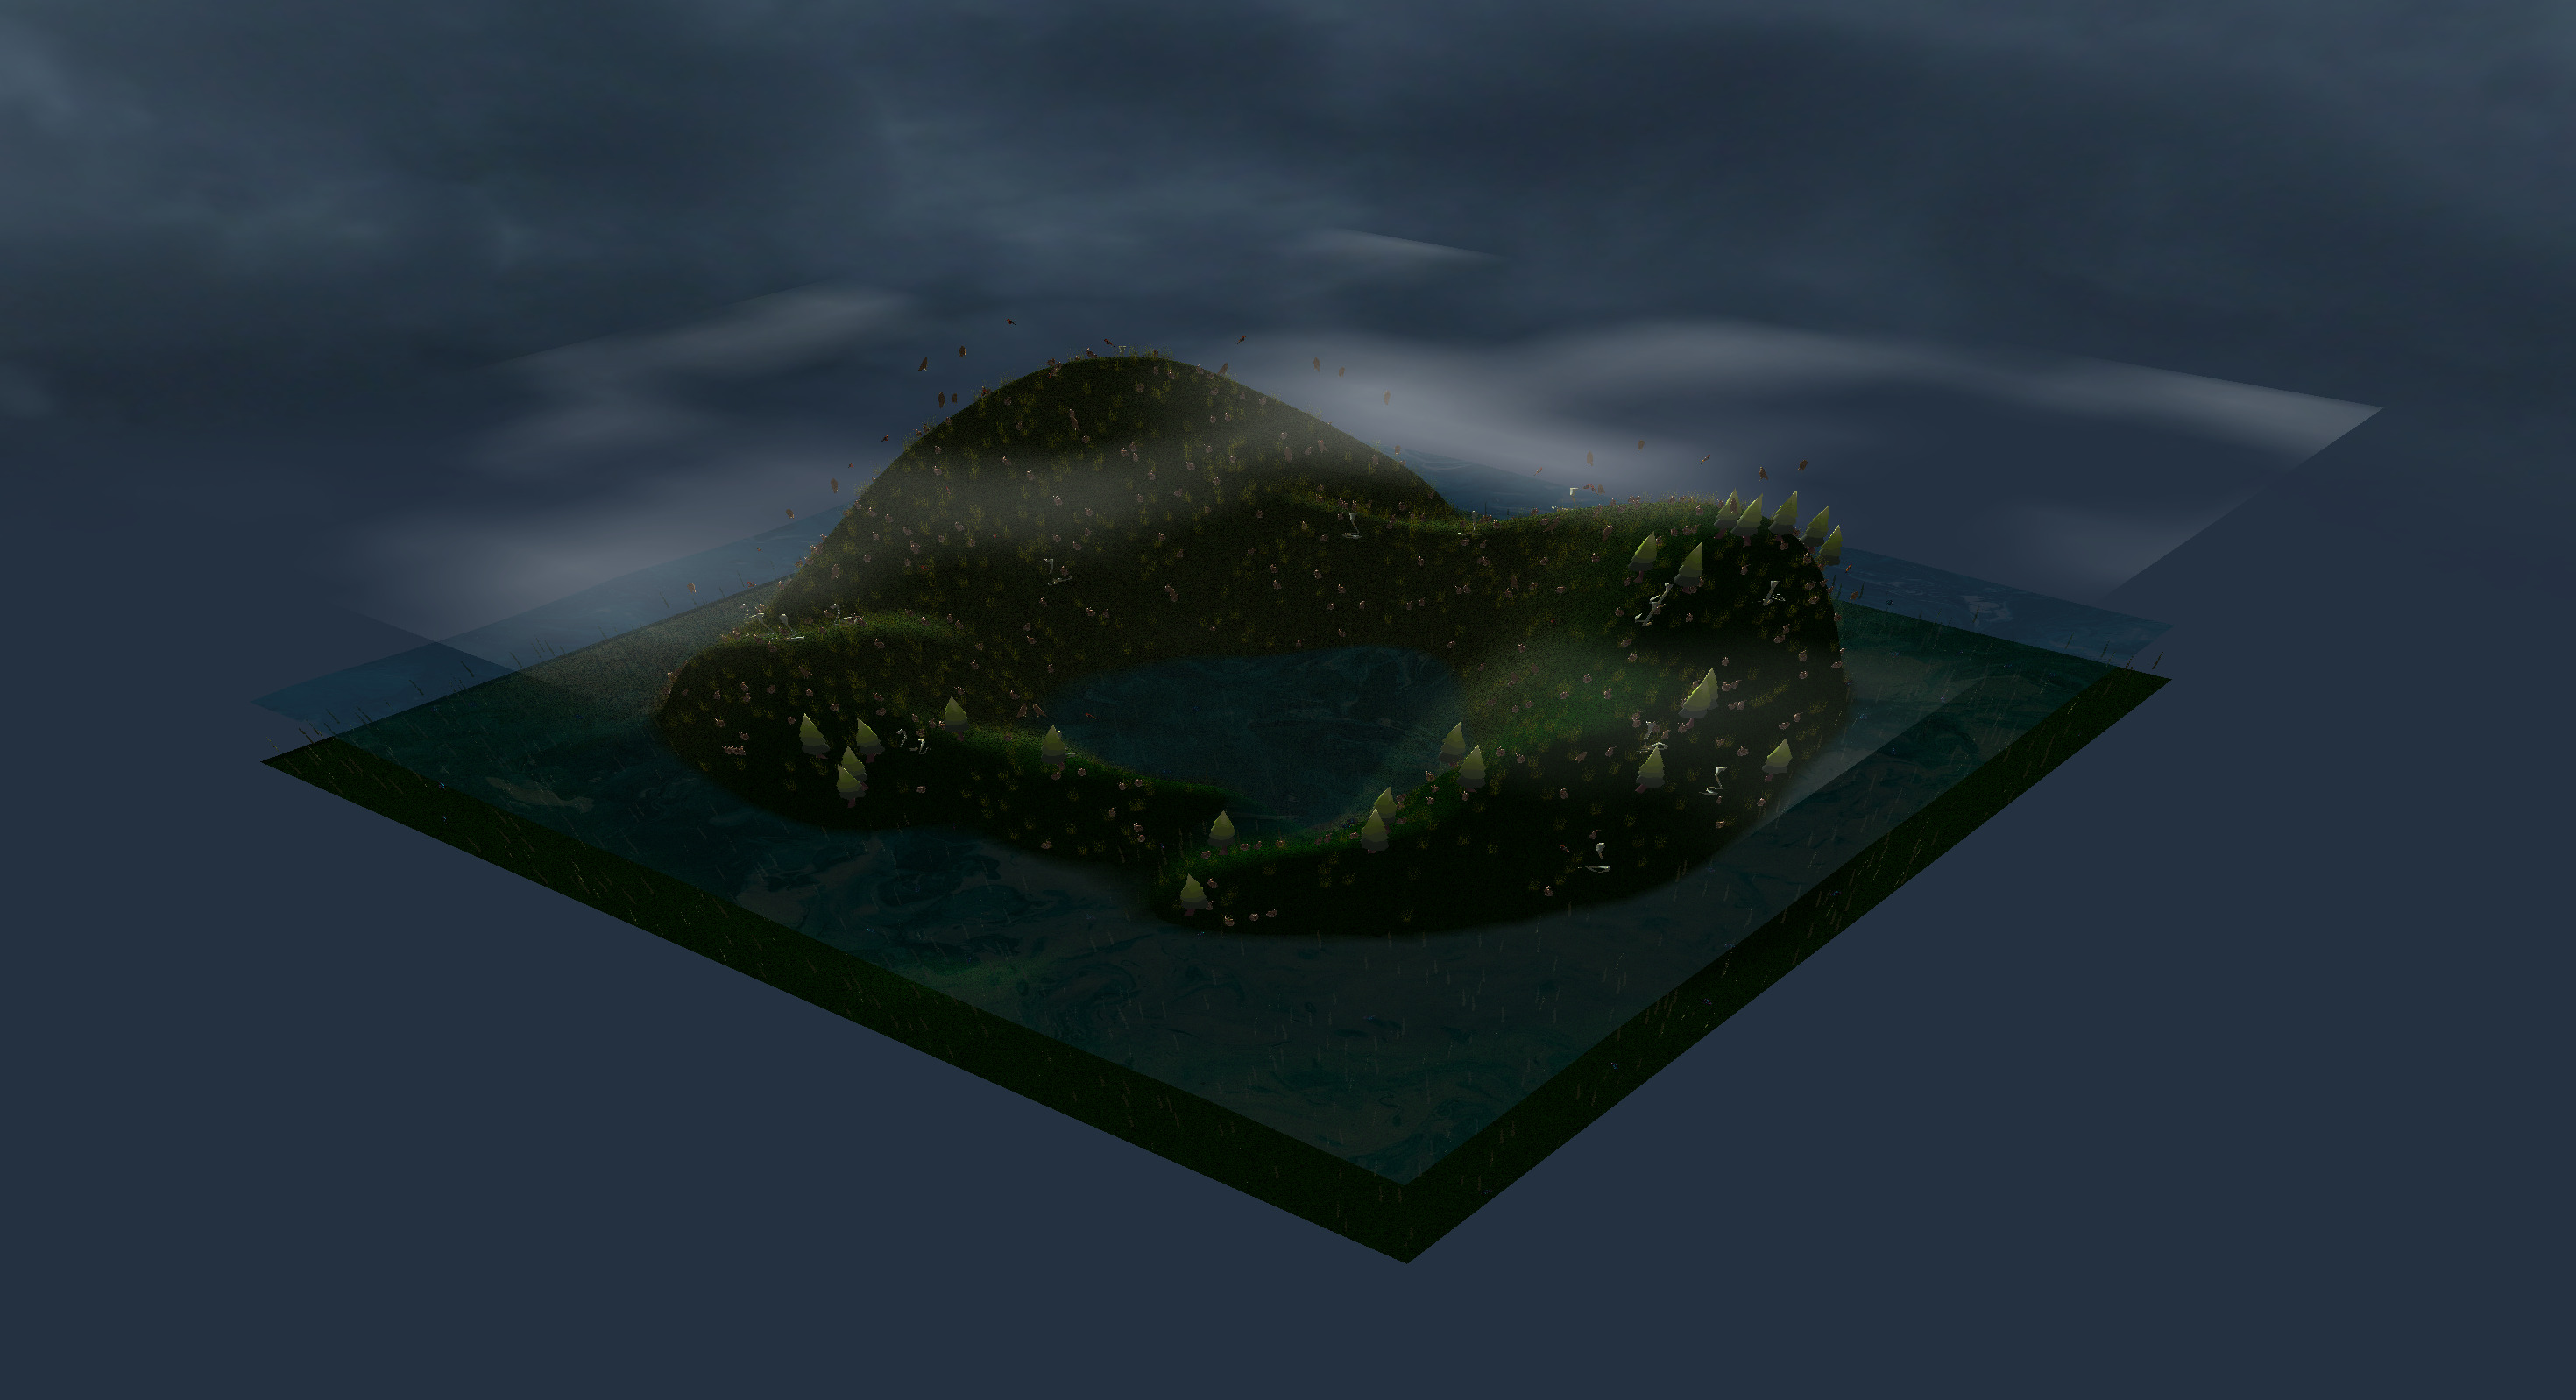
\includegraphics[width=\textwidth]{../screenshots/world1.jpg}
        \caption{World Shot 1 / 3} \label{fig:screenshot-world-1}
    \end{figure}
    \begin{figure}
        \centering
        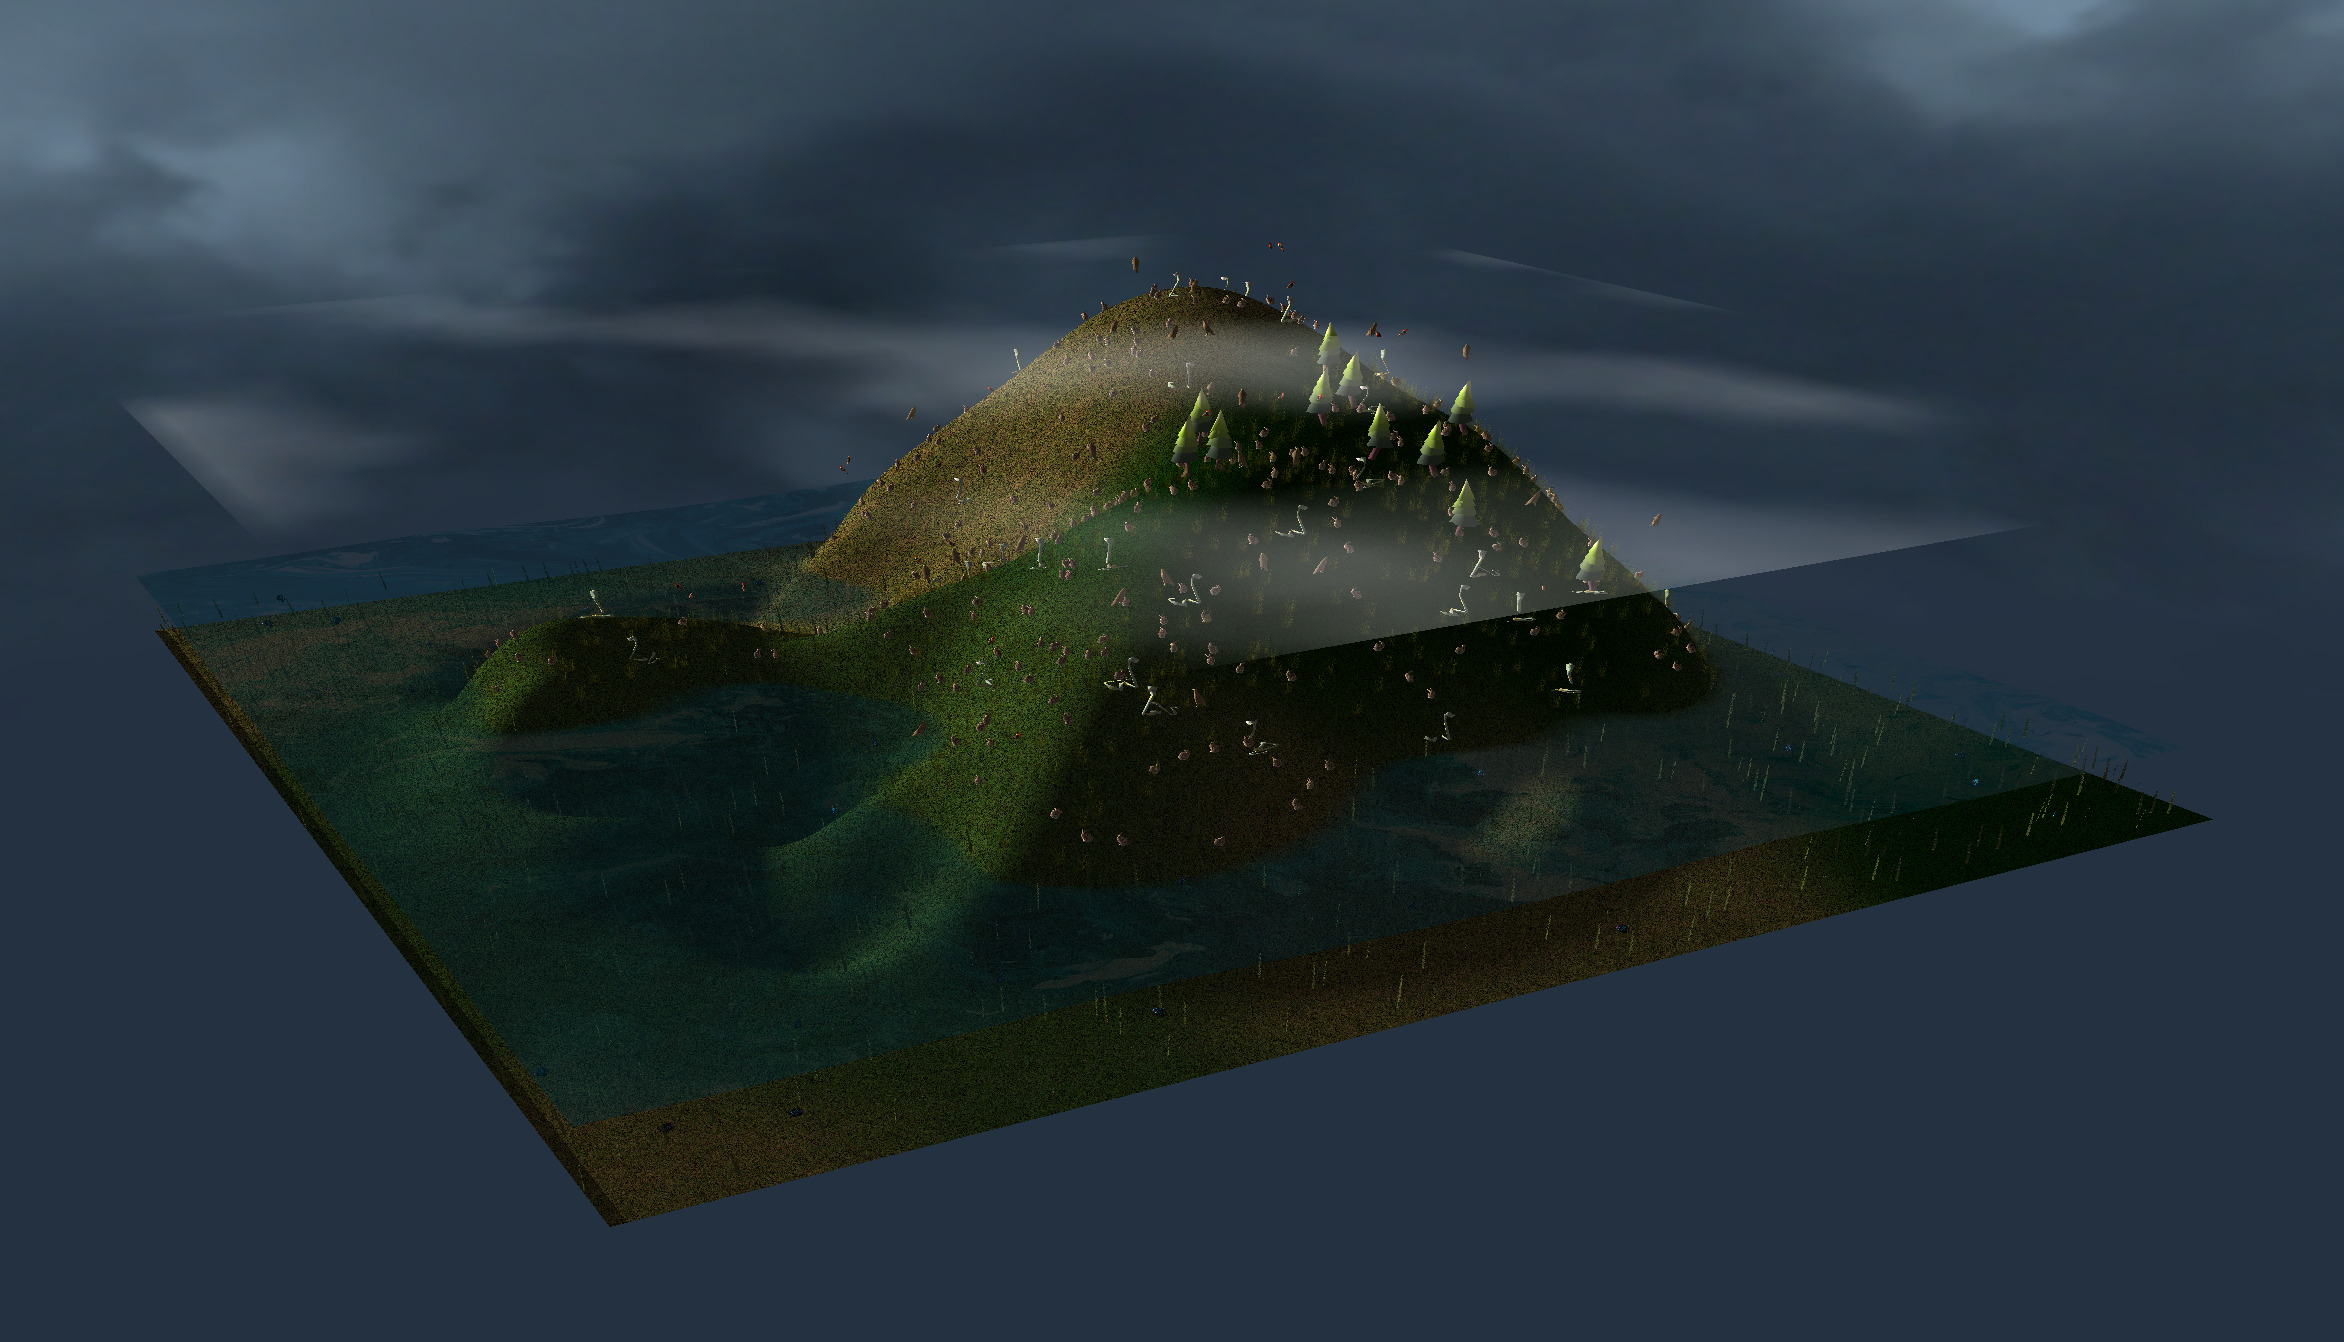
\includegraphics[width=\textwidth]{../screenshots/world2.jpg}
        \caption{World Shot 2 / 3} \label{fig:screenshot-world-2}
    \end{figure}
    \begin{figure}
        \centering
        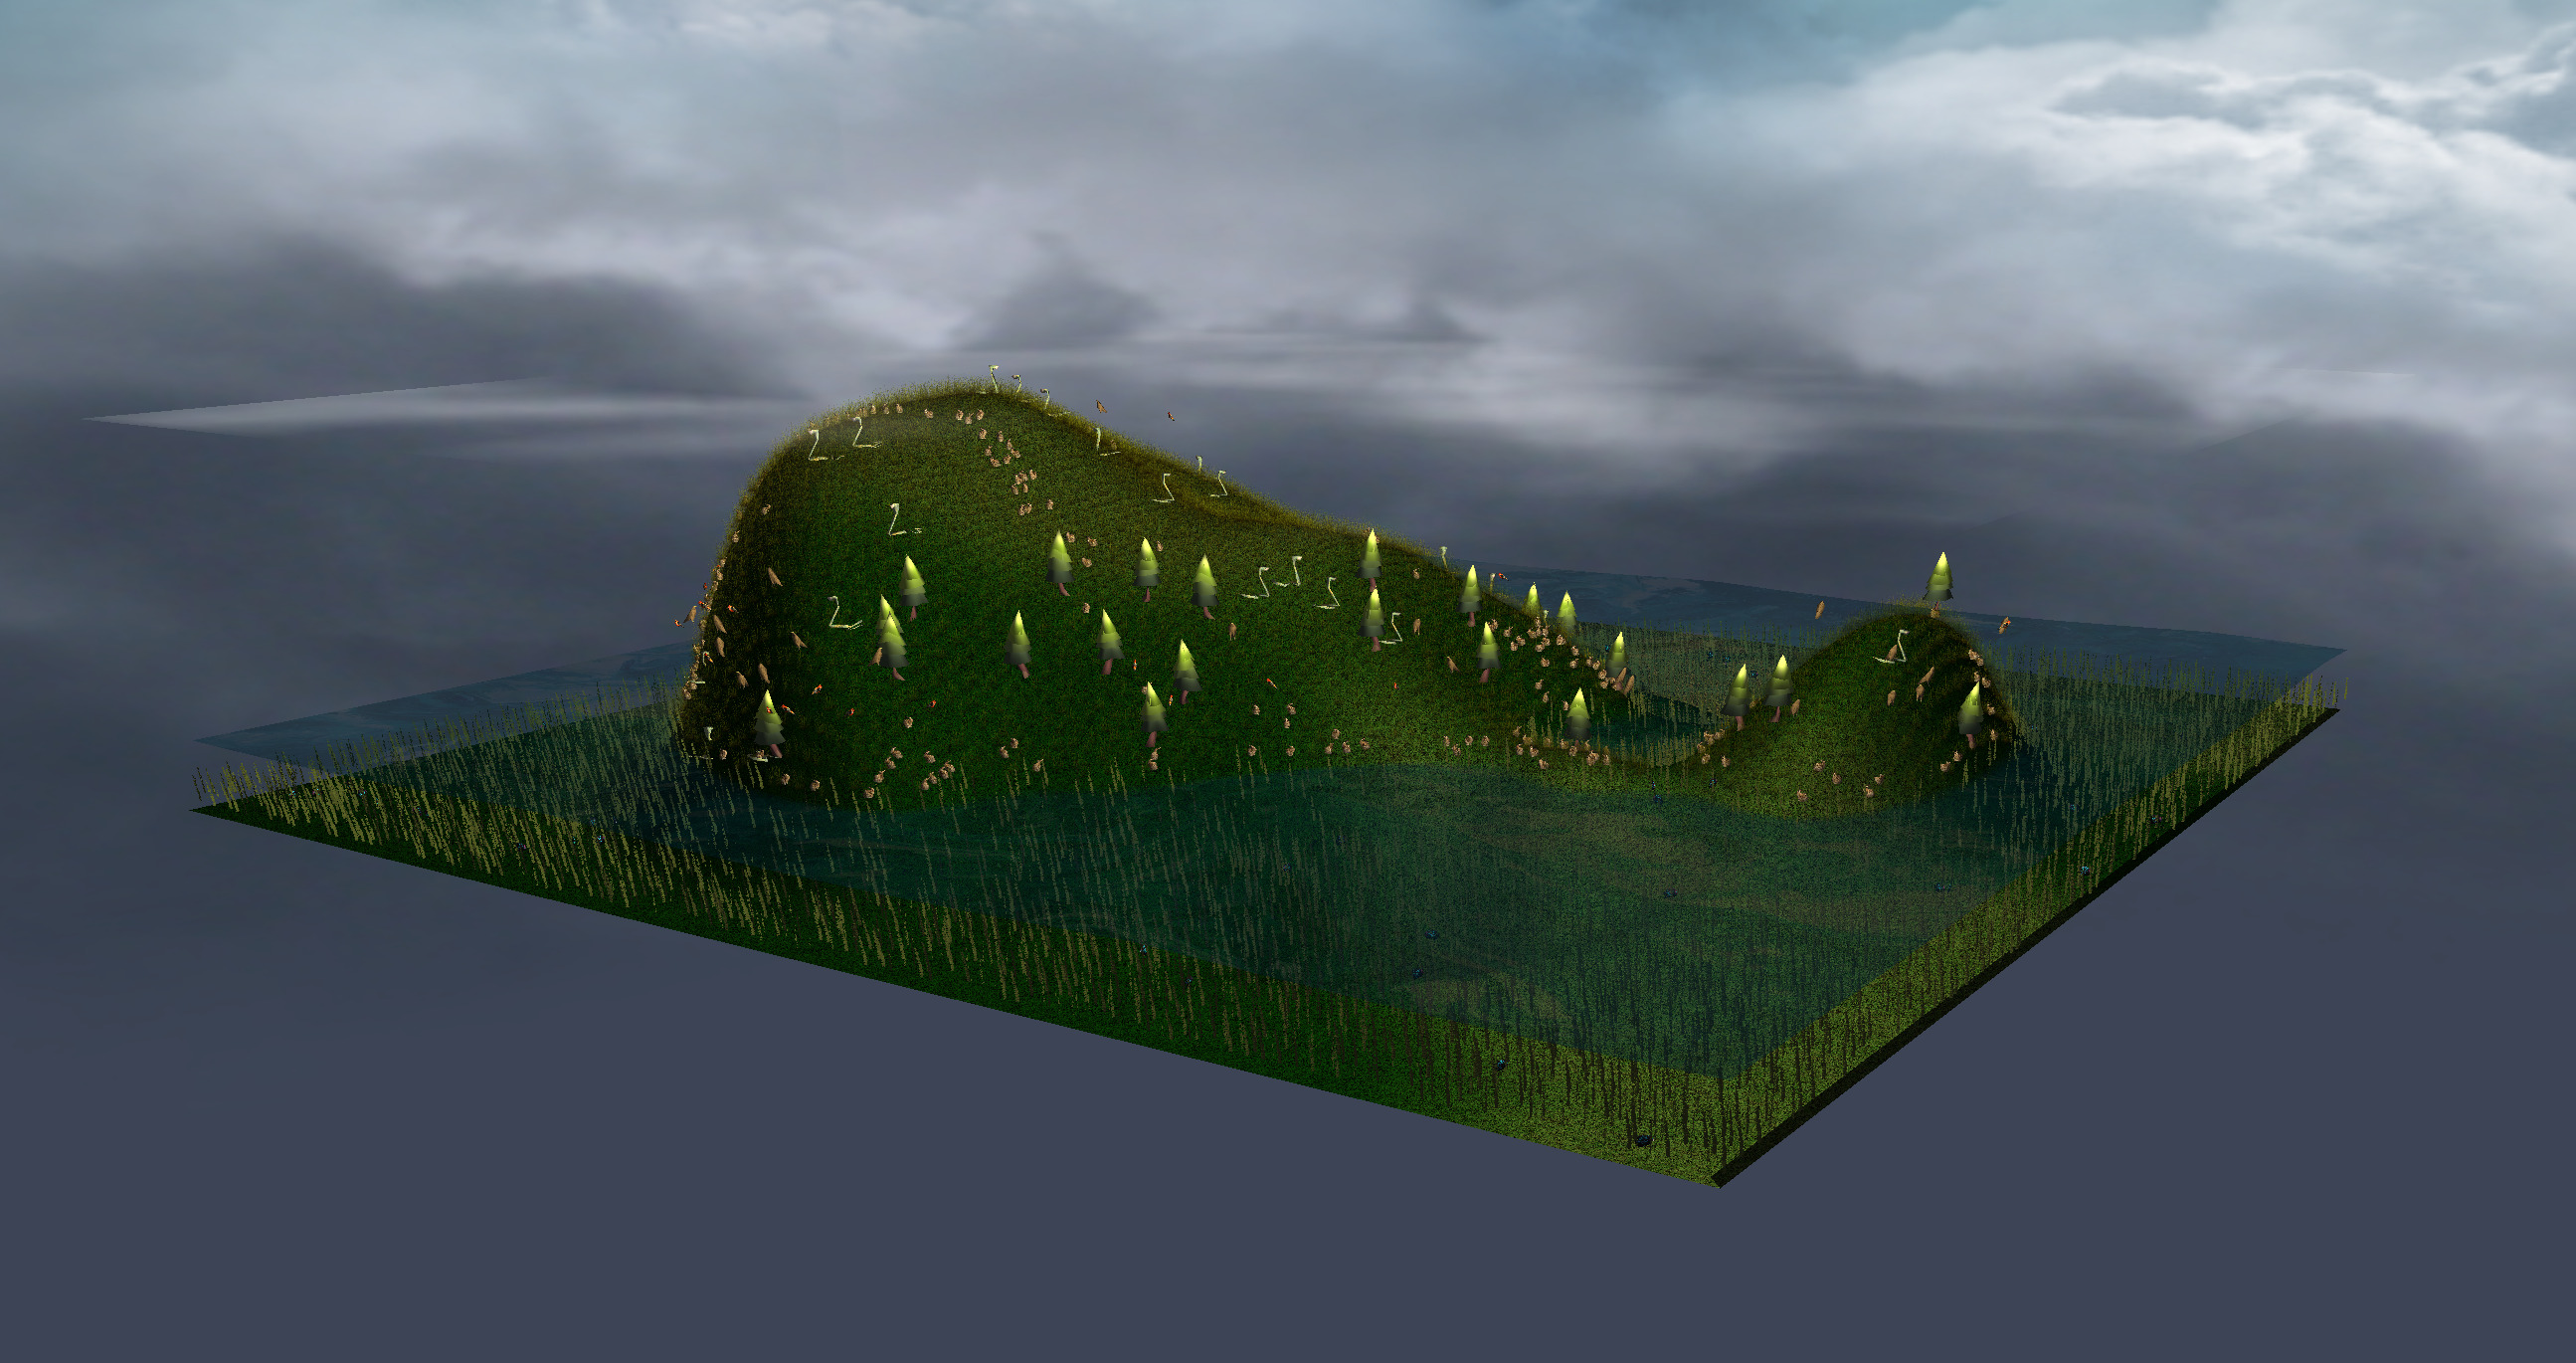
\includegraphics[width=\textwidth]{../screenshots/world3.jpg}
        \caption{World Shot 3 / 3} \label{fig:screenshot-world-3}
    \end{figure}
    \begin{figure}
        \centering
        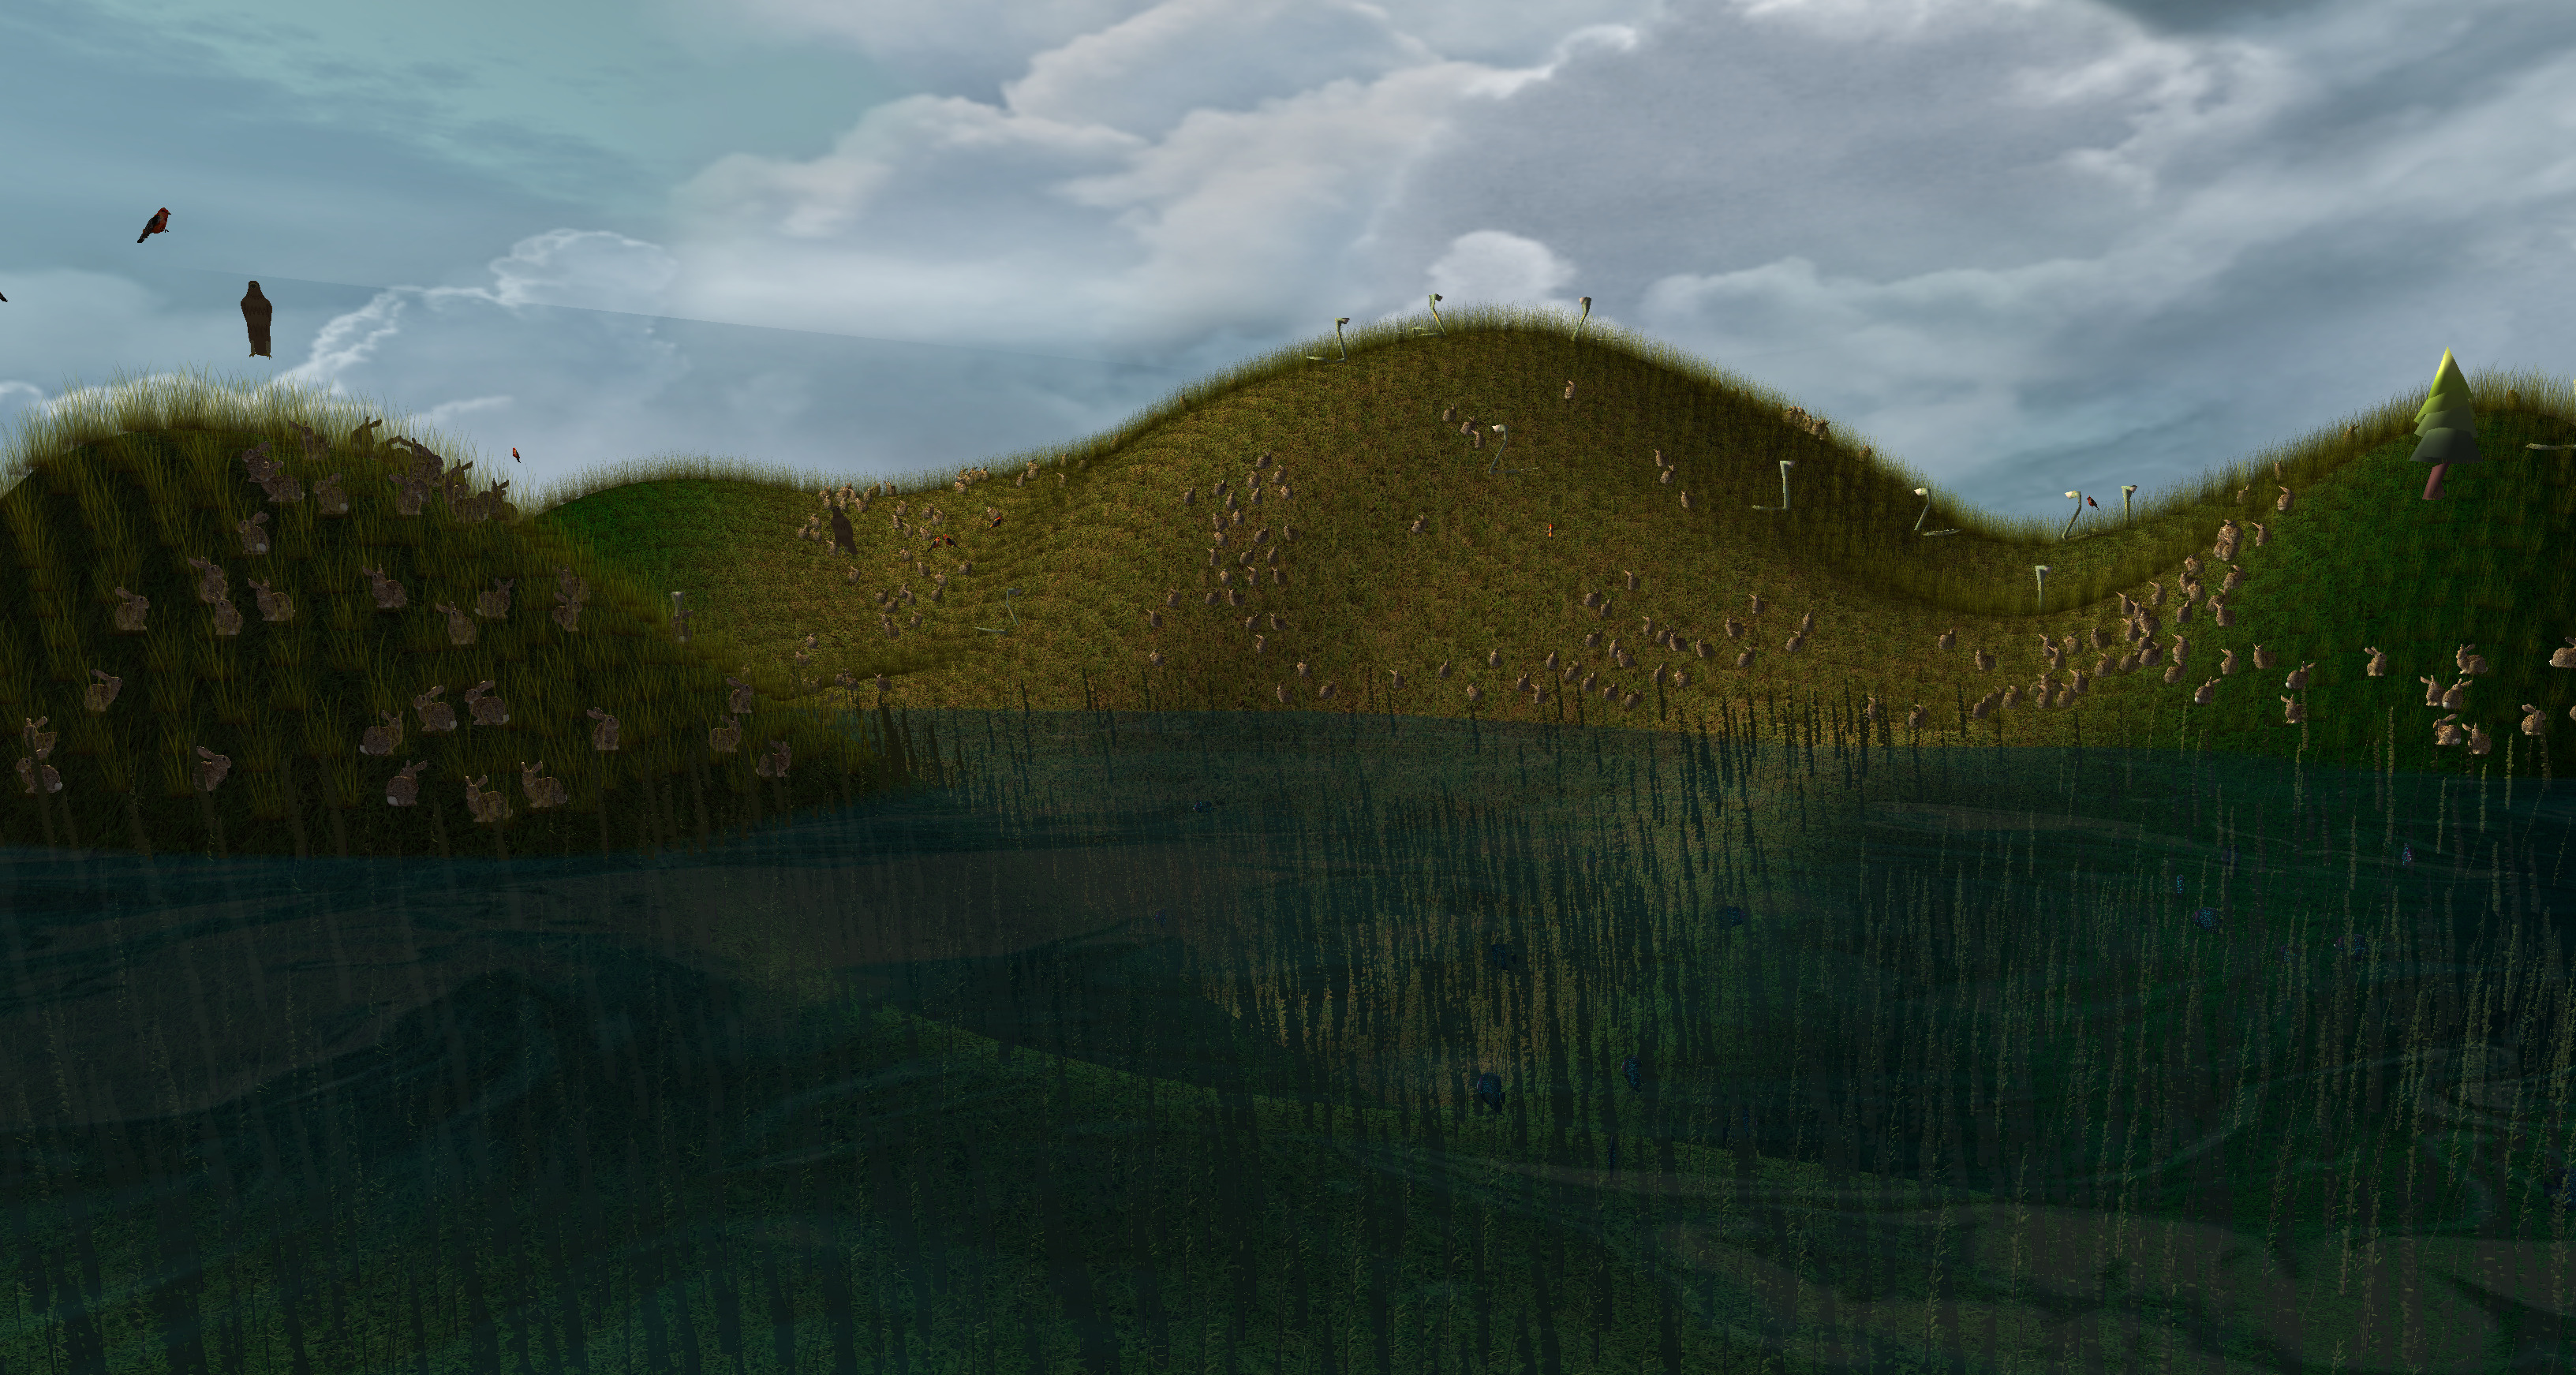
\includegraphics[width=\textwidth]{../screenshots/close1.jpg}
        \caption{Close Shot 1 / 3} \label{fig:screenshot-close-1}
    \end{figure}
    \begin{figure}
        \centering
        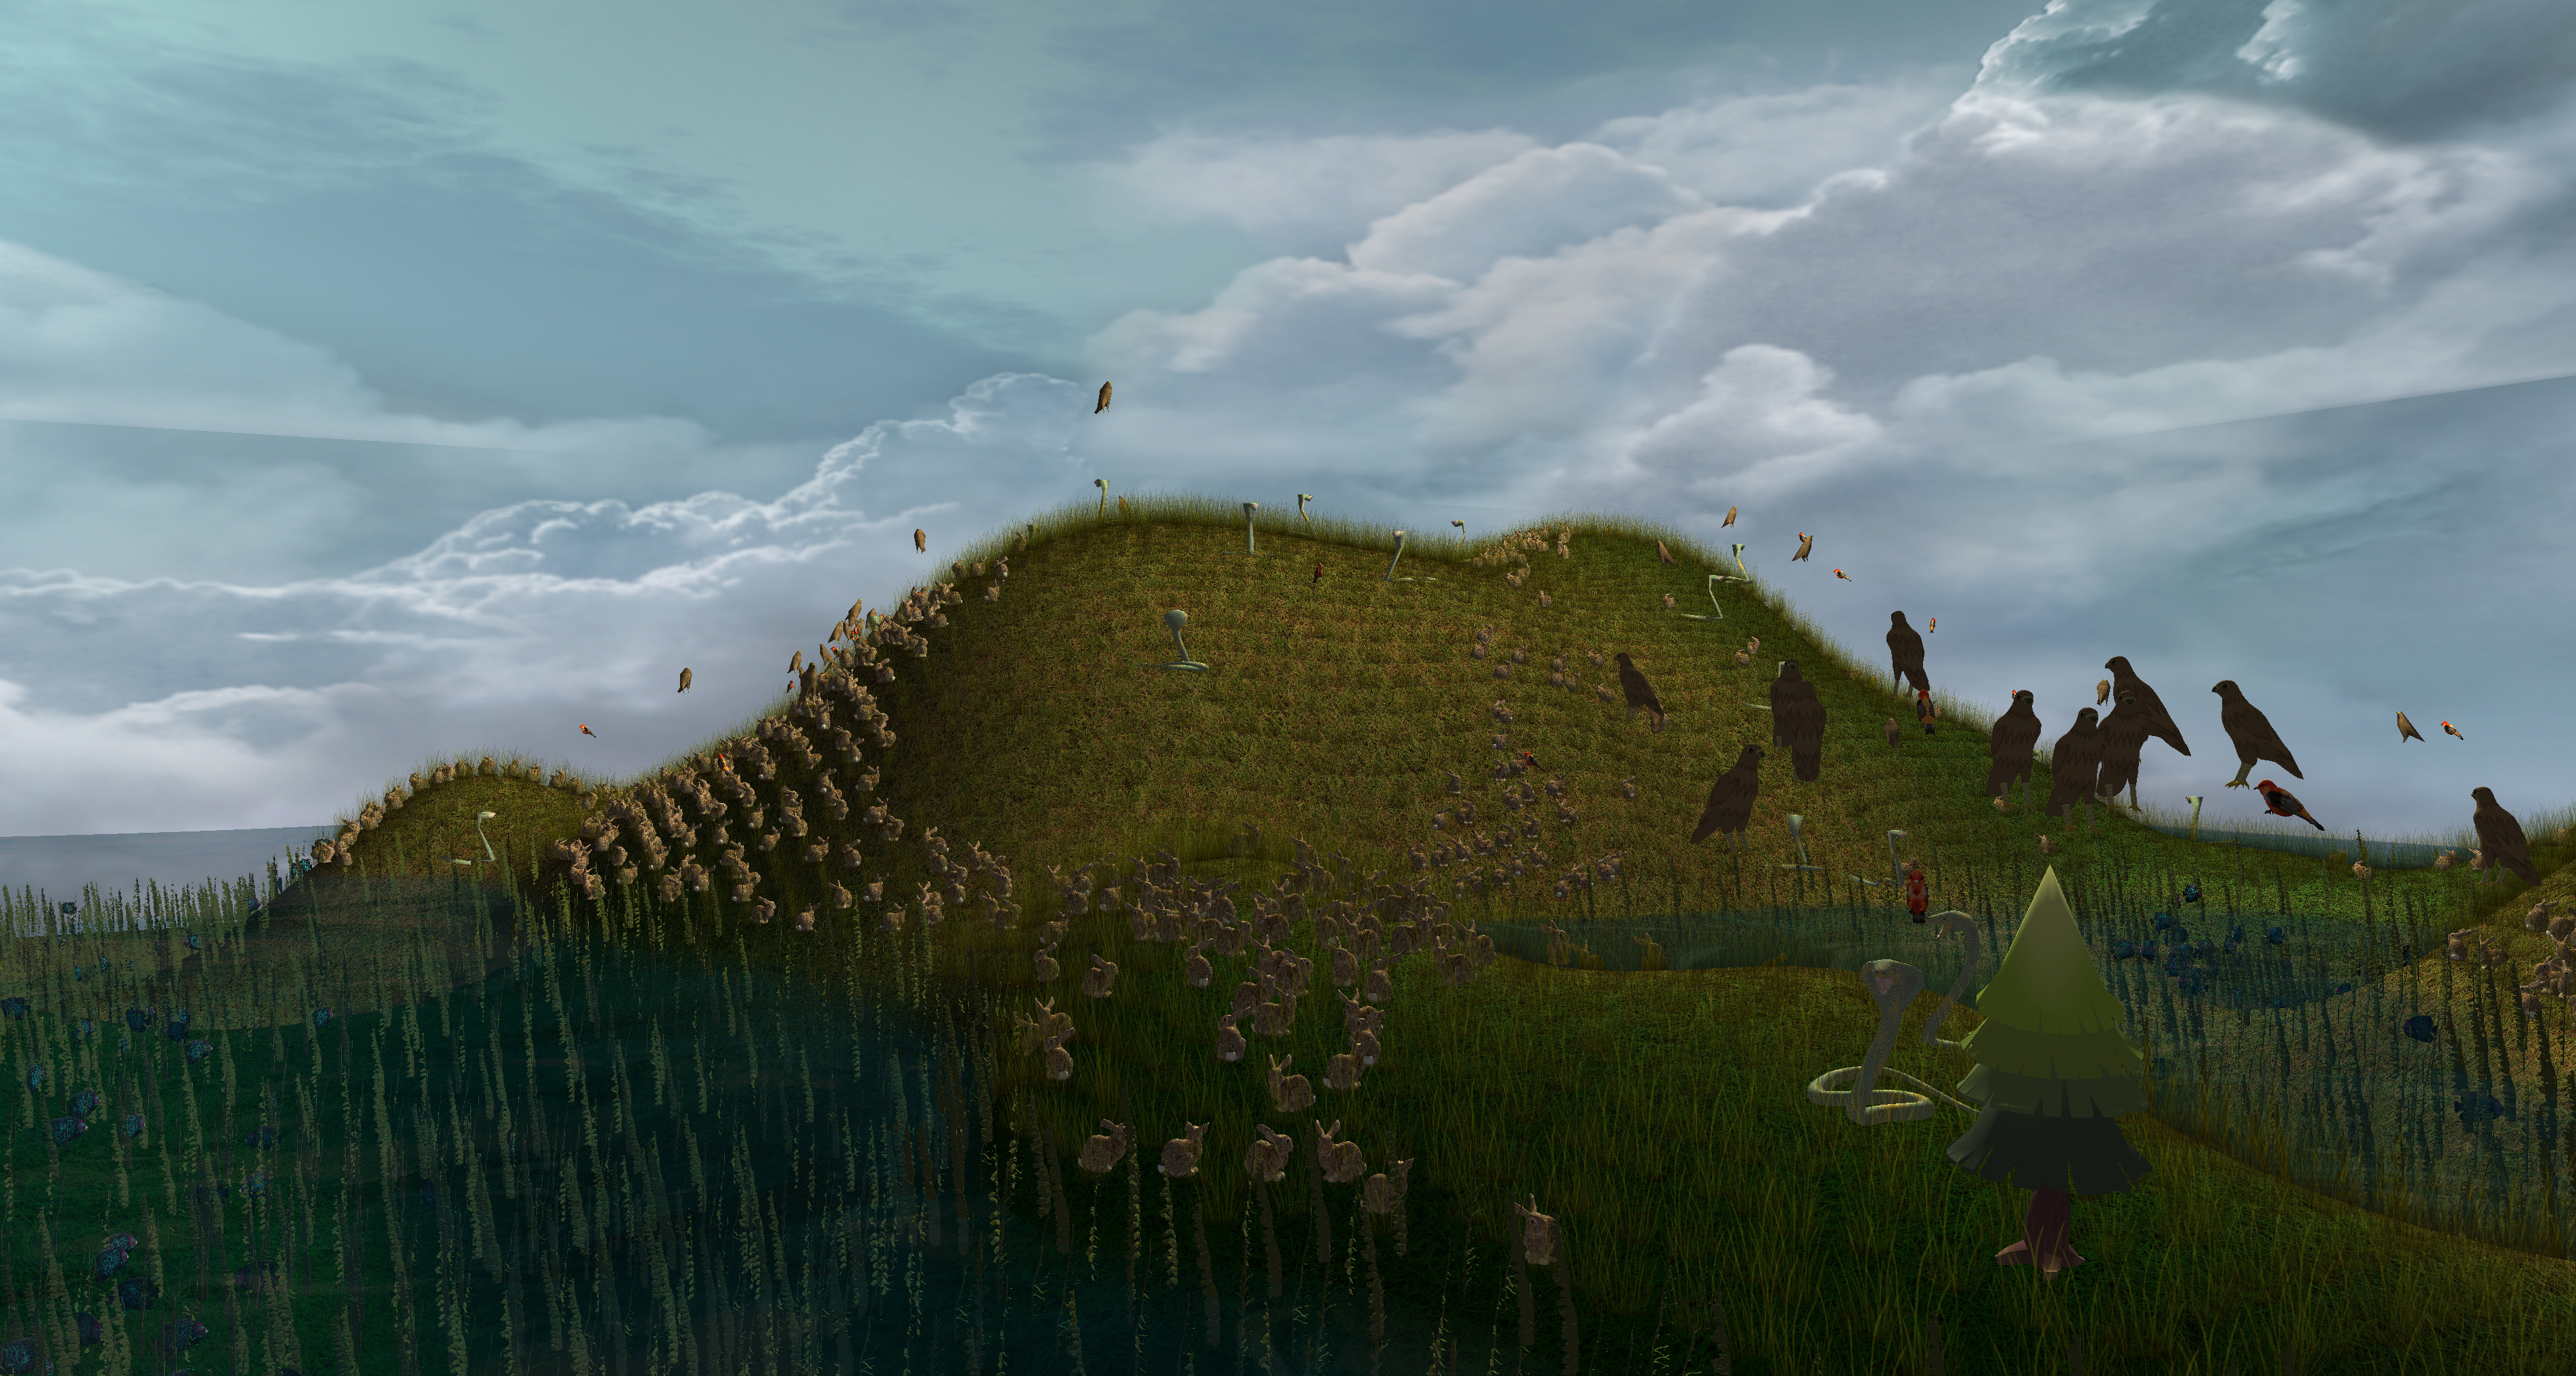
\includegraphics[width=\textwidth]{../screenshots/close2.jpg}
        \caption{Close Shot 2 / 3} \label{fig:screenshot-close-2}
    \end{figure}
    \begin{figure}
        \centering
        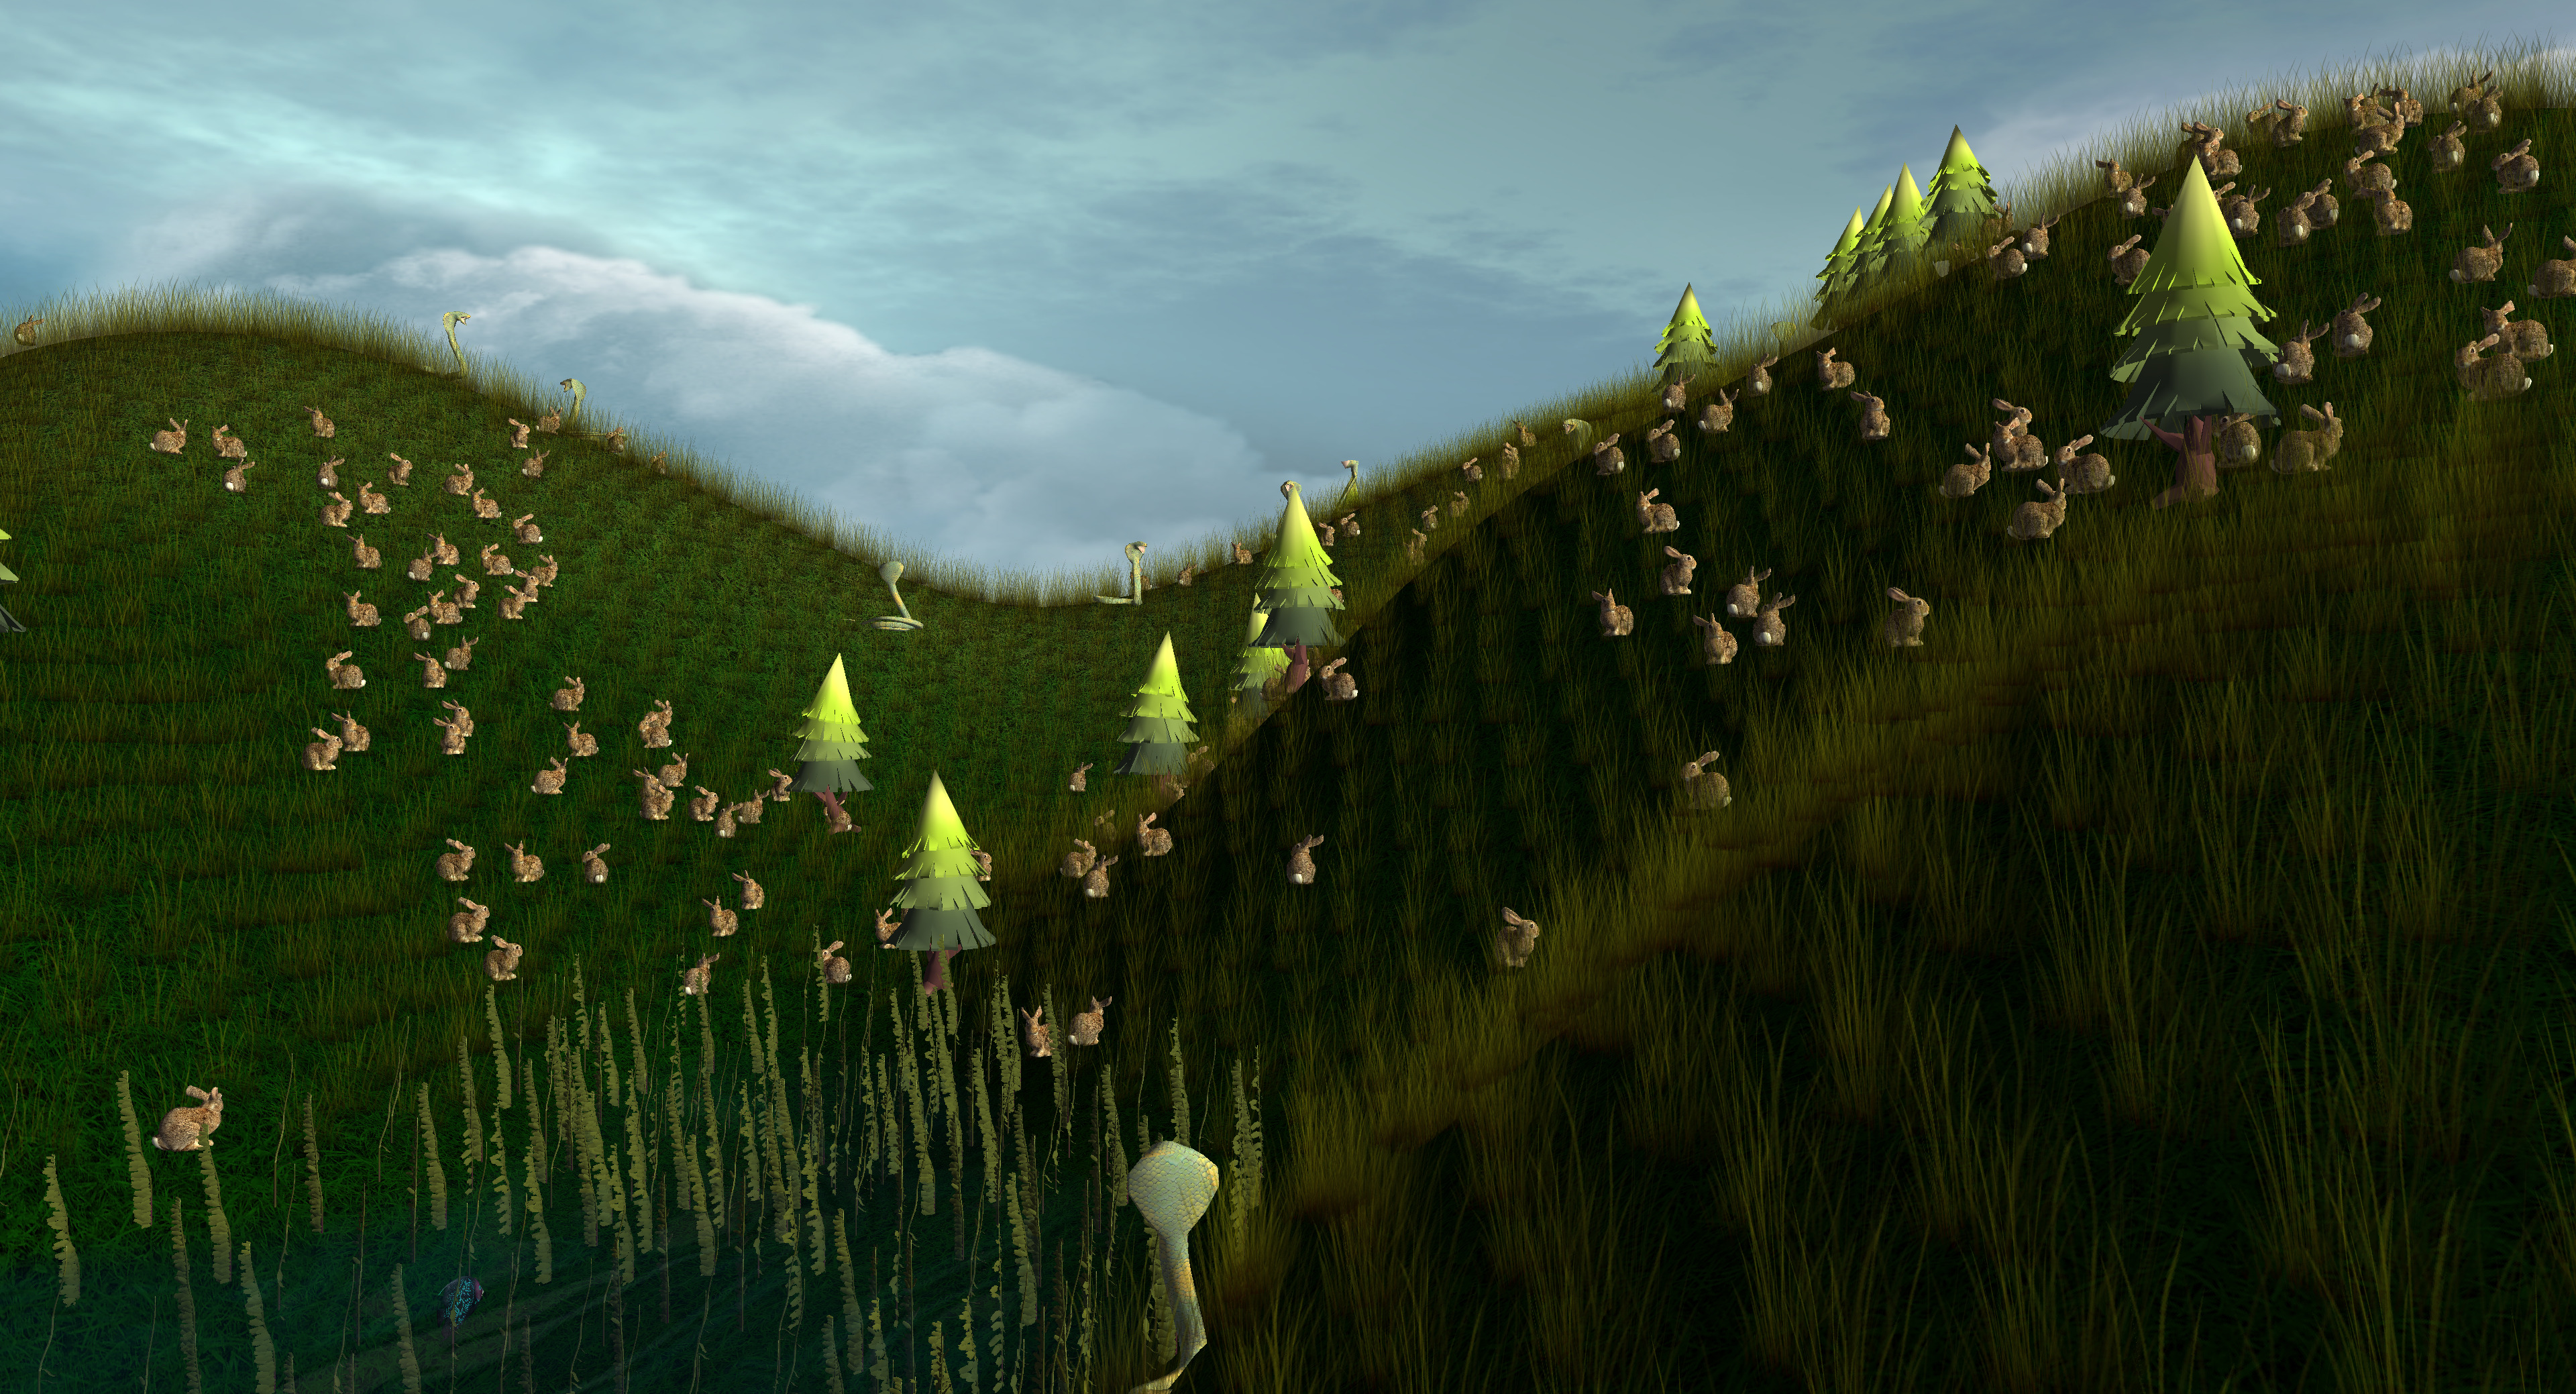
\includegraphics[width=\textwidth]{../screenshots/close3.jpg}
        \caption{Close Shot 3 / 3} \label{fig:screenshot-close-3}
    \end{figure}
    \begin{figure}
        \centering
        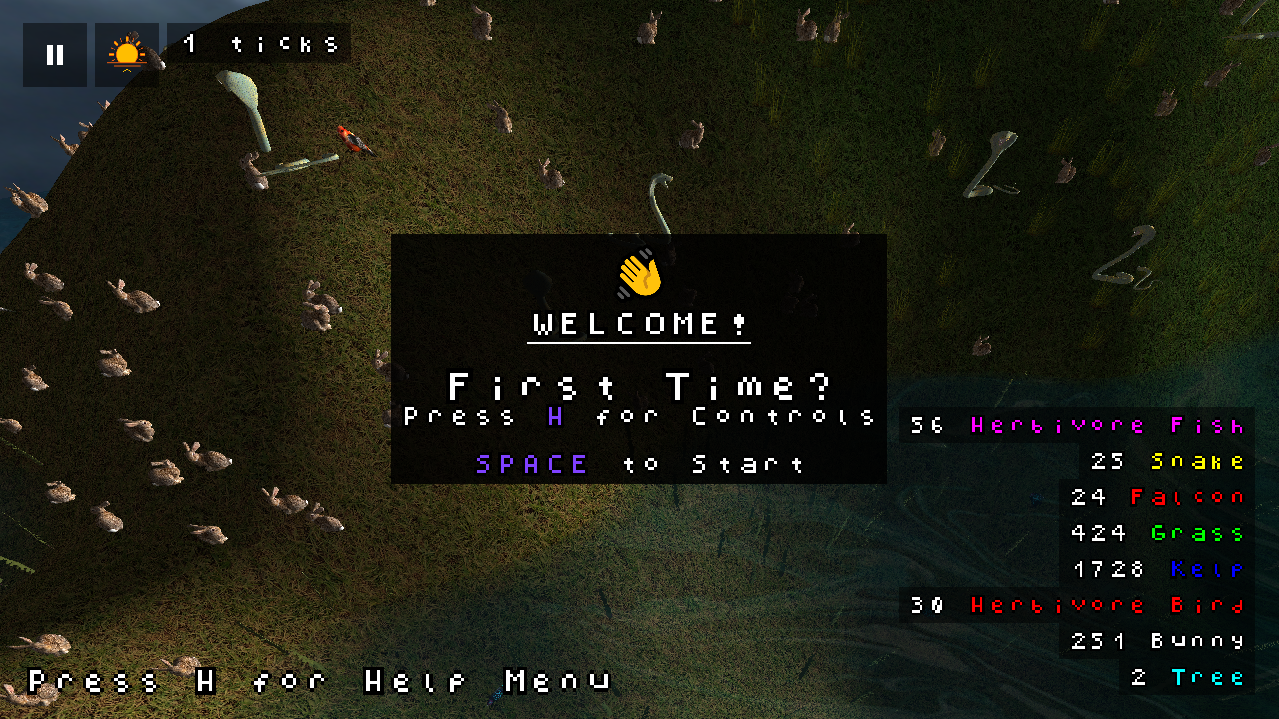
\includegraphics[width=\textwidth]{../screenshots/ui-welcome.png}
        \caption{UI: Welcome Screen} \label{fig:screenshot-ui-welcome}
    \end{figure}
    \begin{figure}
        \centering
        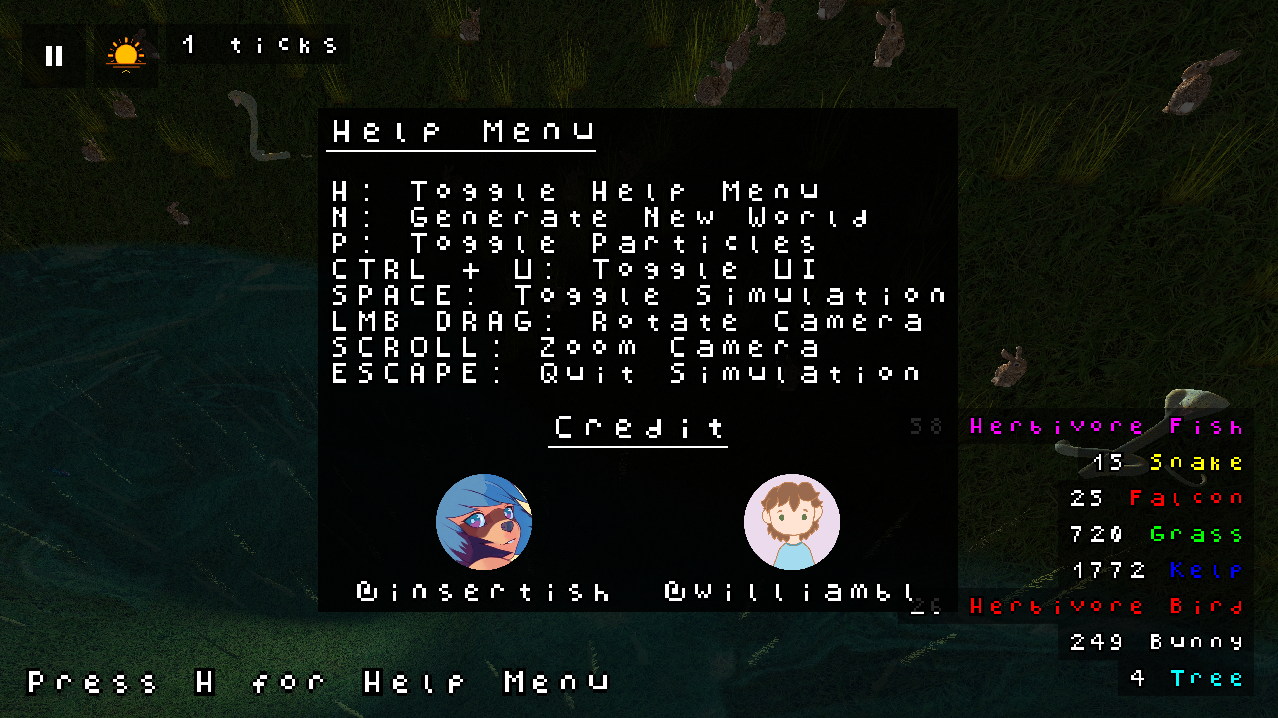
\includegraphics[width=\textwidth]{../screenshots/ui-help.png}
        \caption{UI: Help Menu} \label{fig:screenshot-ui-help}
    \end{figure}
    \begin{figure}
        \centering
        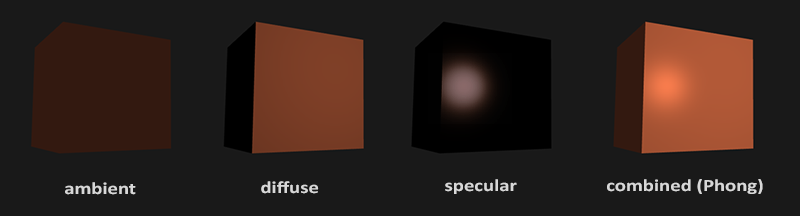
\includegraphics[width=\textwidth]{images/phong.png}
        \caption{Phong Lighting Model \cite{learnopengl-lighting}} \label{fig:phong}
    \end{figure}
    \begin{figure}
        \centering
        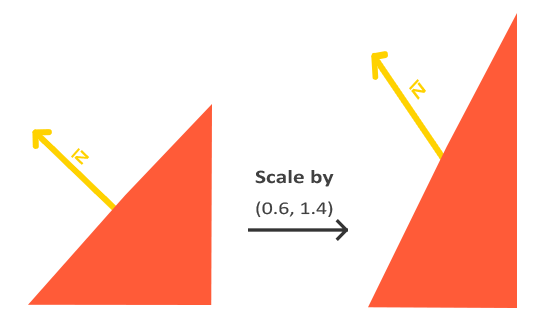
\includegraphics[width=\textwidth]{images/transforming_normals.png}
        \caption{Transforming Normal Vectors \cite{learnopengl-lighting}} \label{fig:normals}
    \end{figure}
    \begin{figure}
        \centering
        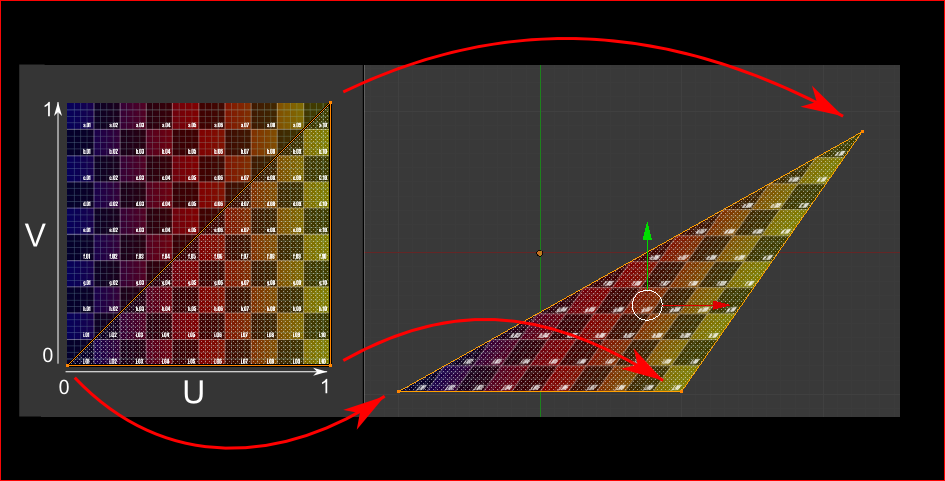
\includegraphics[width=\textwidth]{images/opengluv.png}
        \caption{OpenGL UV mapping \cite{opengl-tutorial-textured-cube}} \label{fig:uvmapping}
    \end{figure}
    \begin{figure}
        \centering
        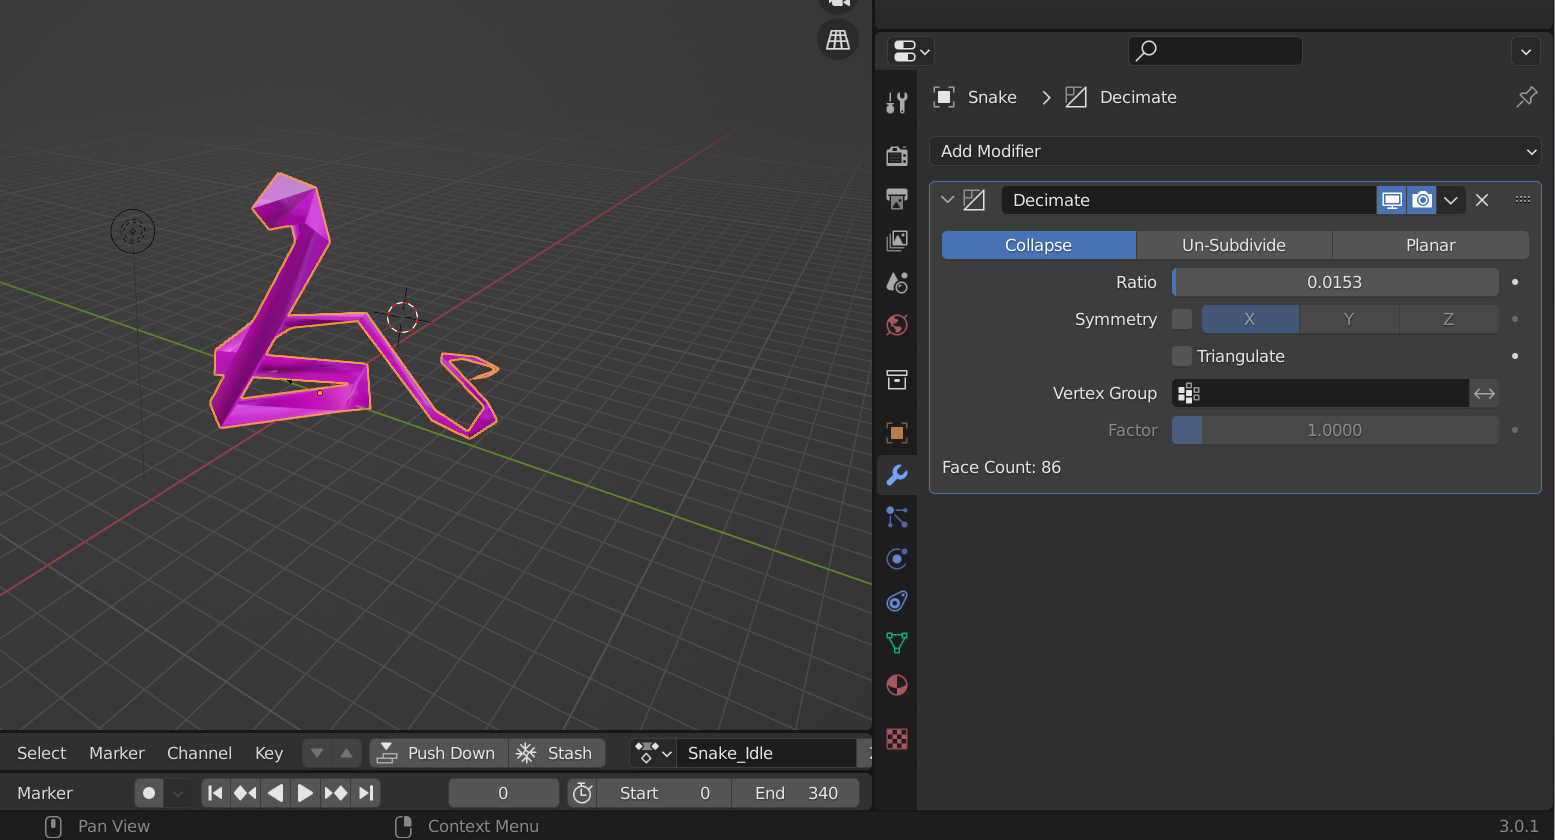
\includegraphics[width=\textwidth]{images/decimate.png}
        \caption{Decimate Filter in Blender} \label{fig:decimate}
    \end{figure}
    \begin{figure}
        \centering
        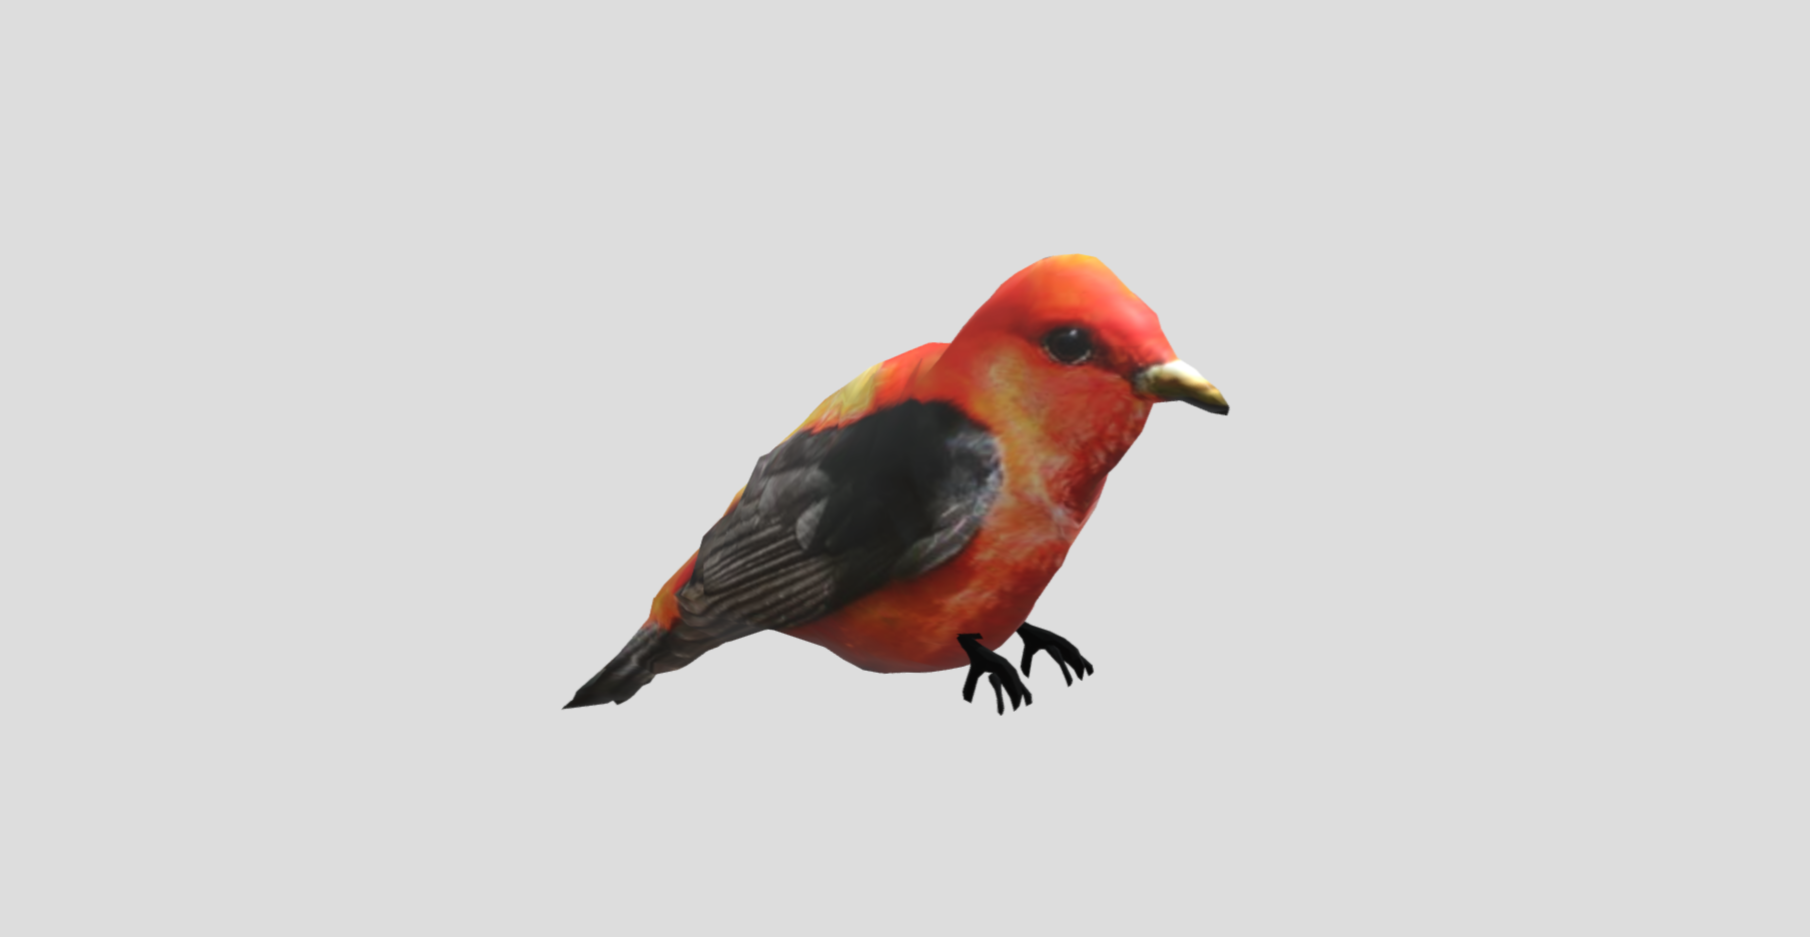
\includegraphics[width=\textwidth]{images/models/bird.png}
        \caption{Bird Model \cite{model-bird}} \label{fig:bird-model}
    \end{figure}
    \begin{figure}
        \centering
        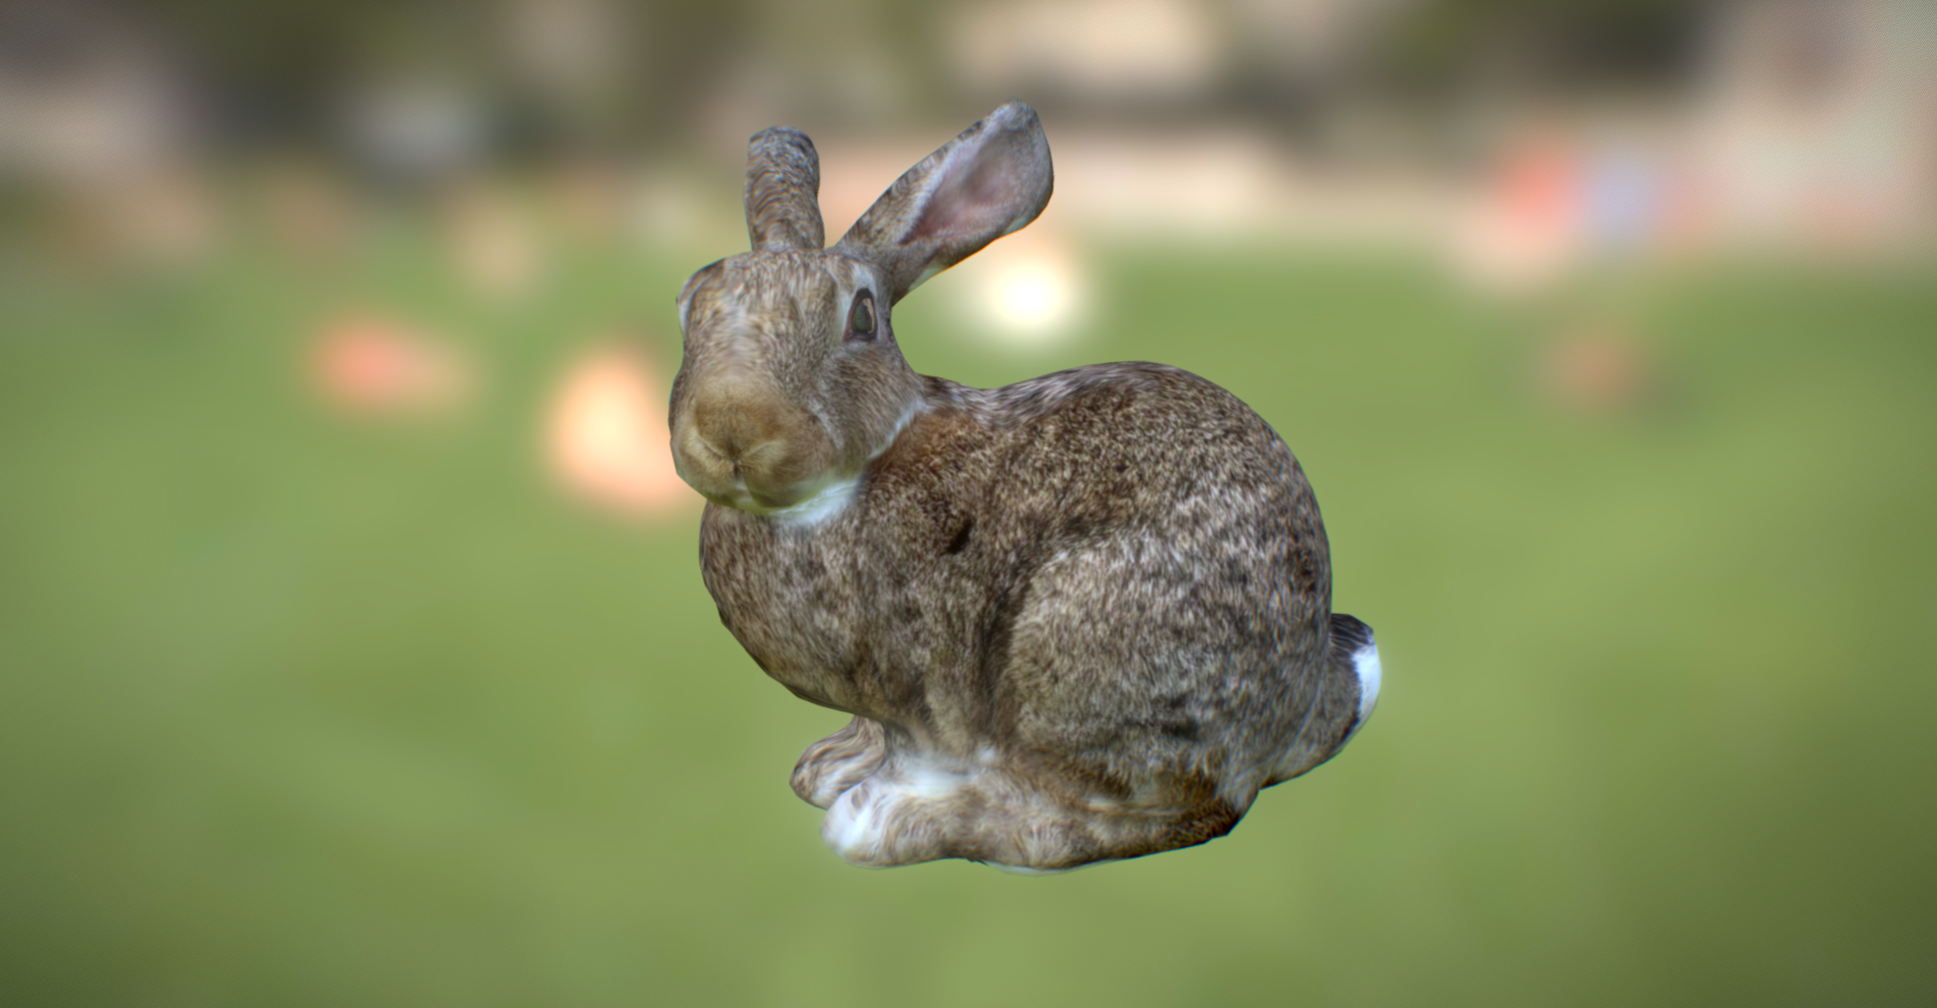
\includegraphics[width=\textwidth]{images/models/bunny.png}
        \caption{Bunny Model \cite{model-bunny}} \label{fig:bunny-model}
    \end{figure}
    \begin{figure}
        \centering
        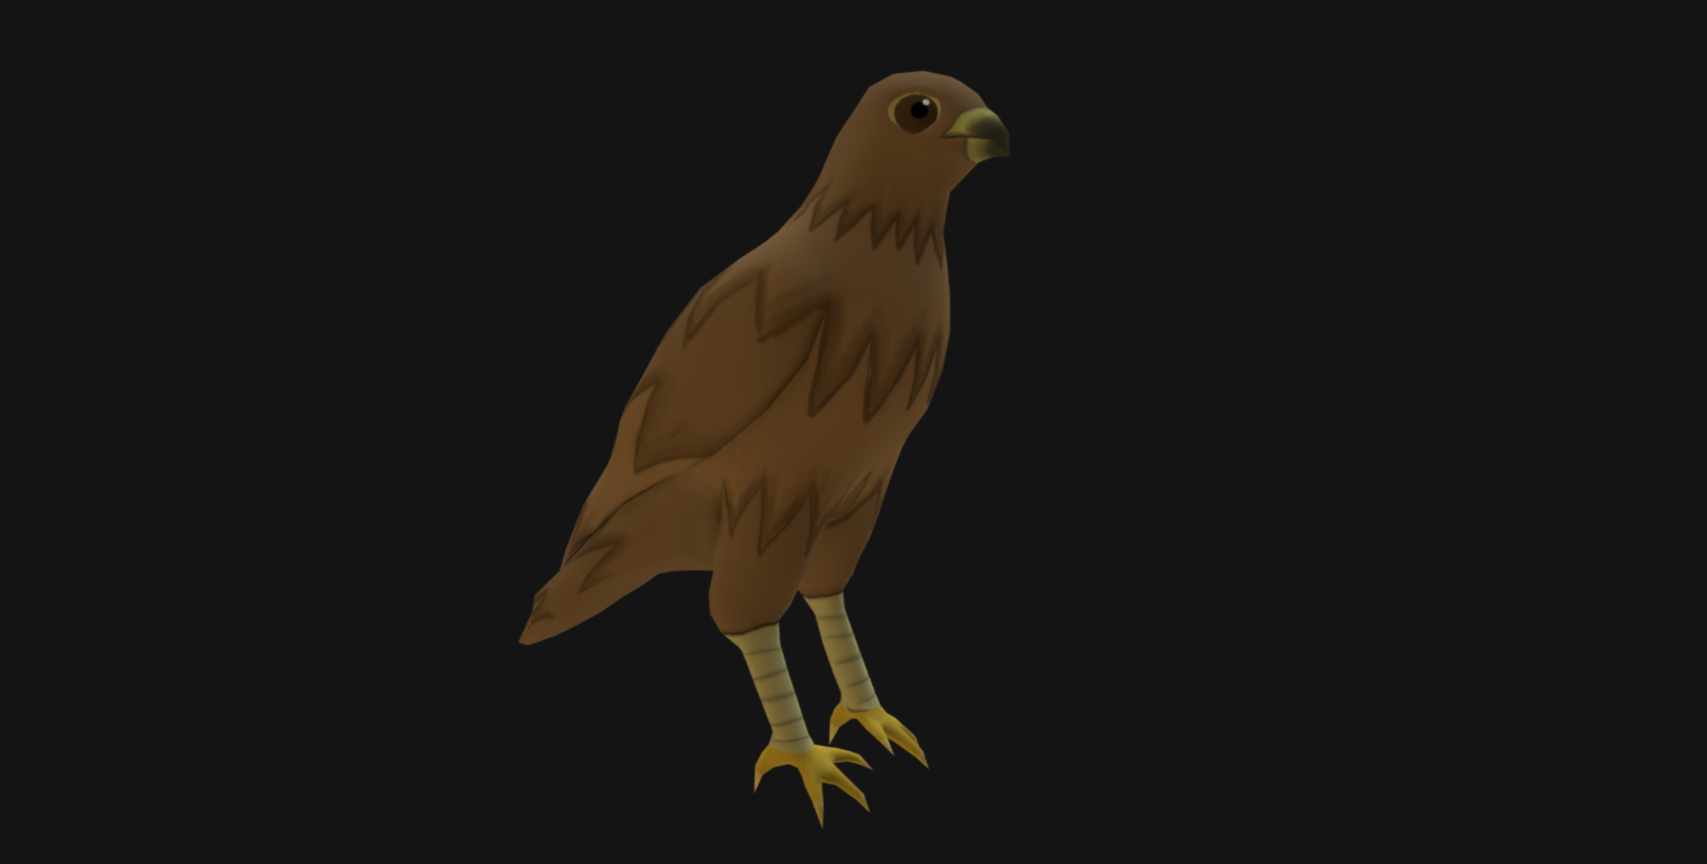
\includegraphics[width=\textwidth]{images/models/falcon.png}
        \caption{Falcon Model \cite{model-falcon}} \label{fig:falcon-model}
    \end{figure}
    \begin{figure}
        \centering
        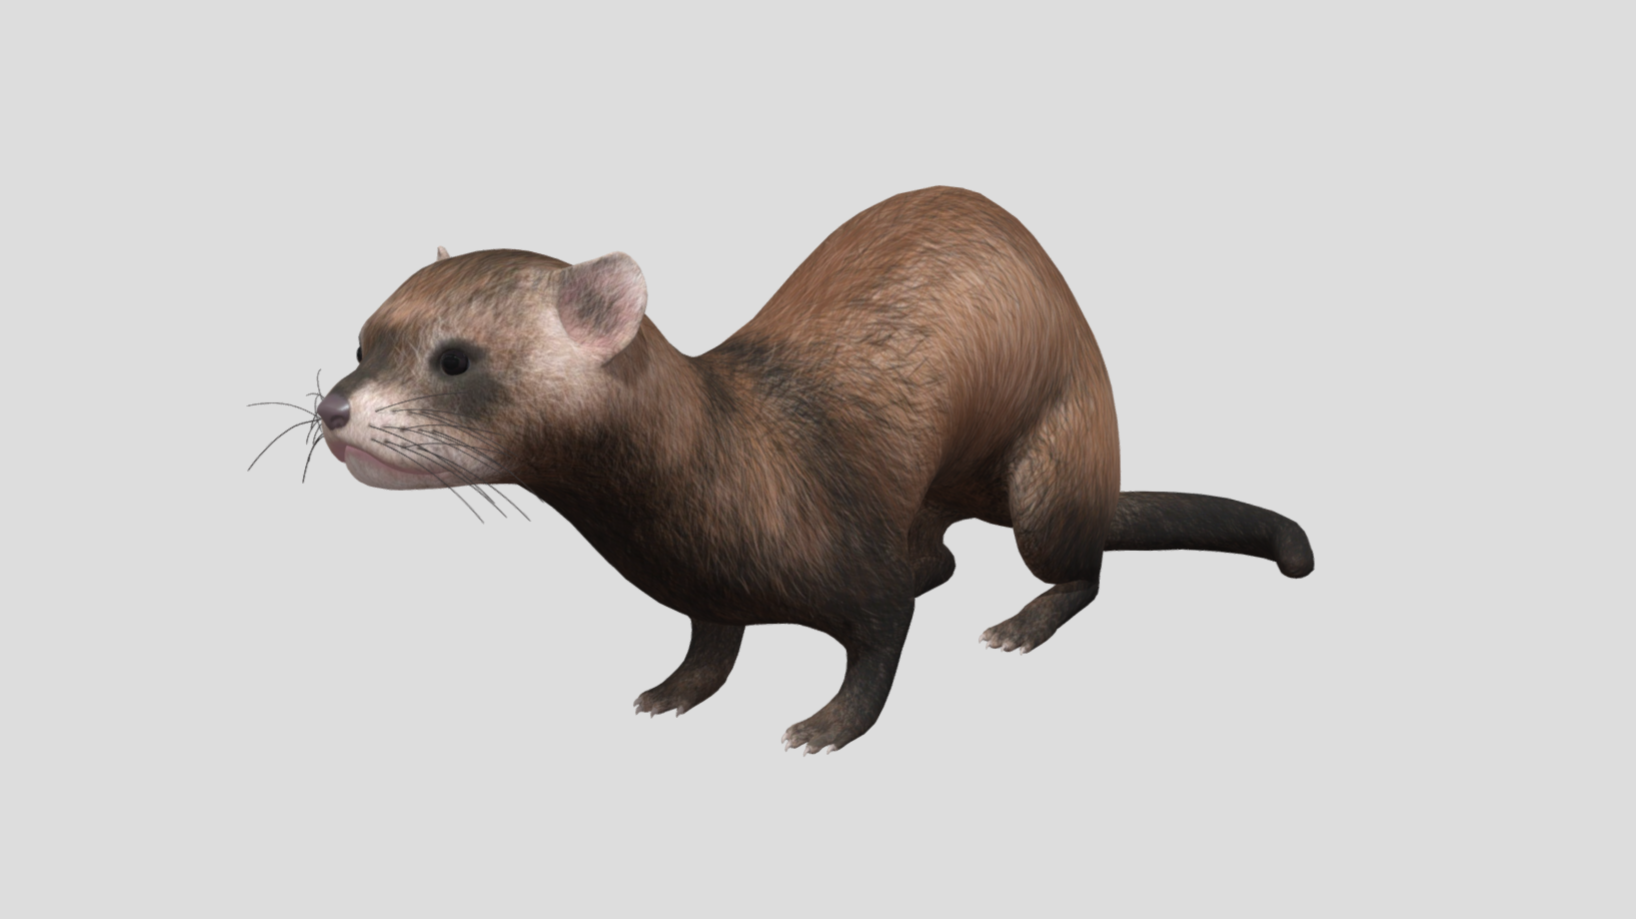
\includegraphics[width=\textwidth]{images/models/ferret.png}
        \caption{Ferret Model \cite{model-ferret}} \label{fig:ferret-model}
    \end{figure}
    \begin{figure}
        \centering
        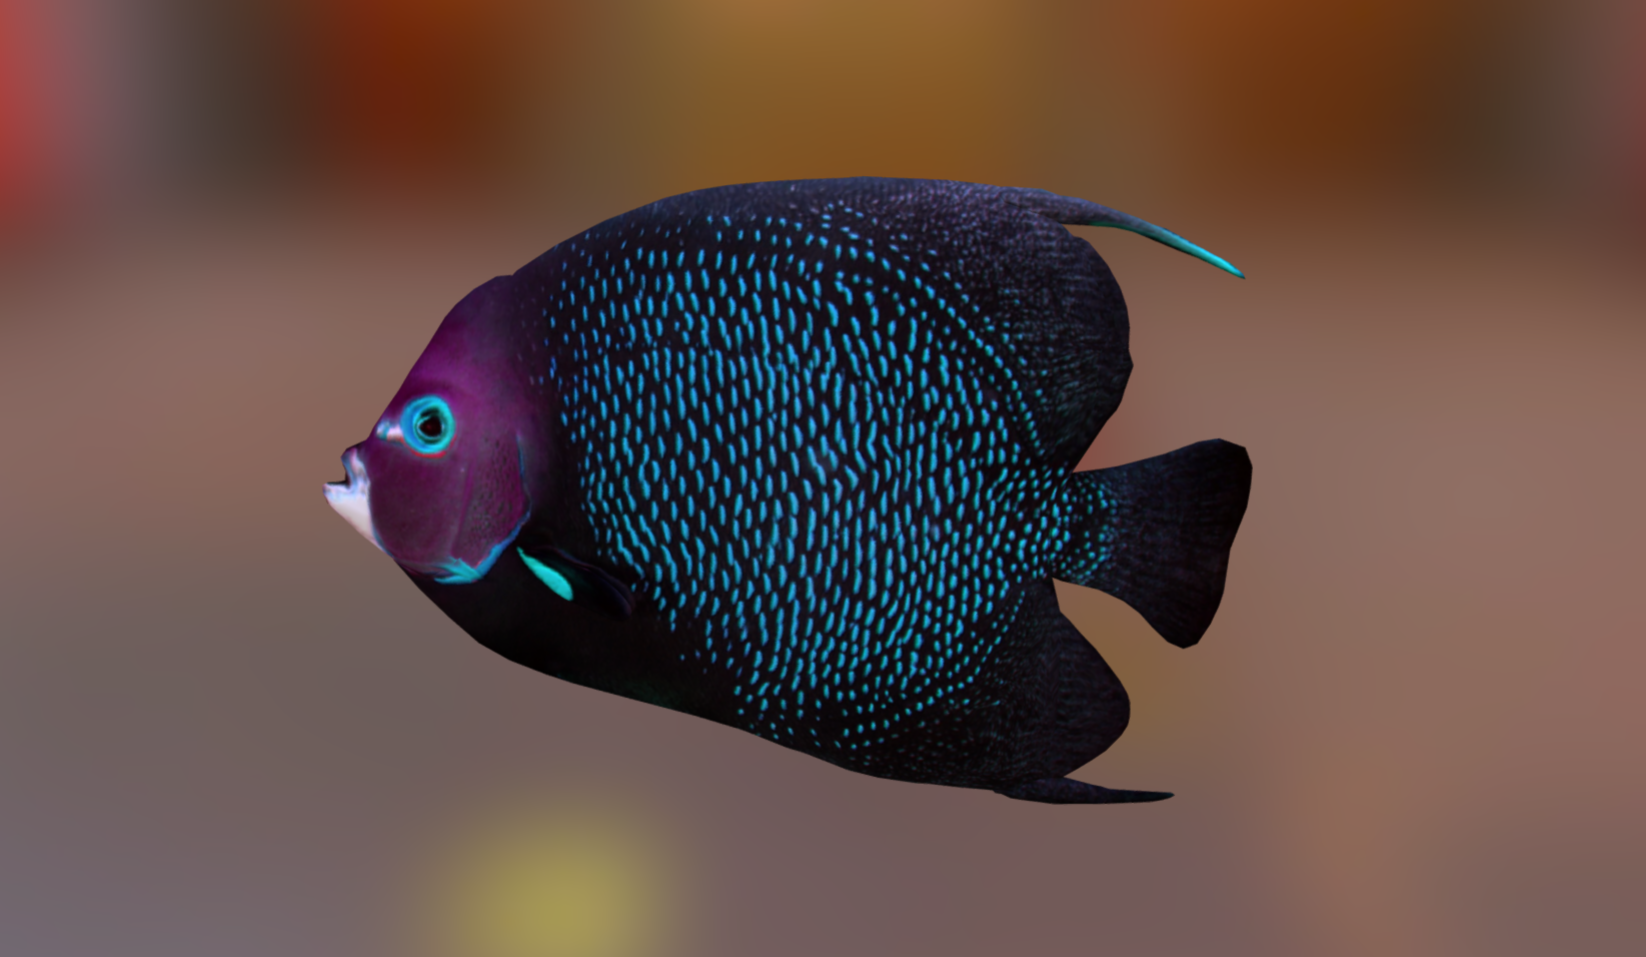
\includegraphics[width=\textwidth]{images/models/fish.png}
        \caption{Fish Model \cite{model-fish}} \label{fig:fish-model}
    \end{figure}
    \begin{figure}
        \centering
        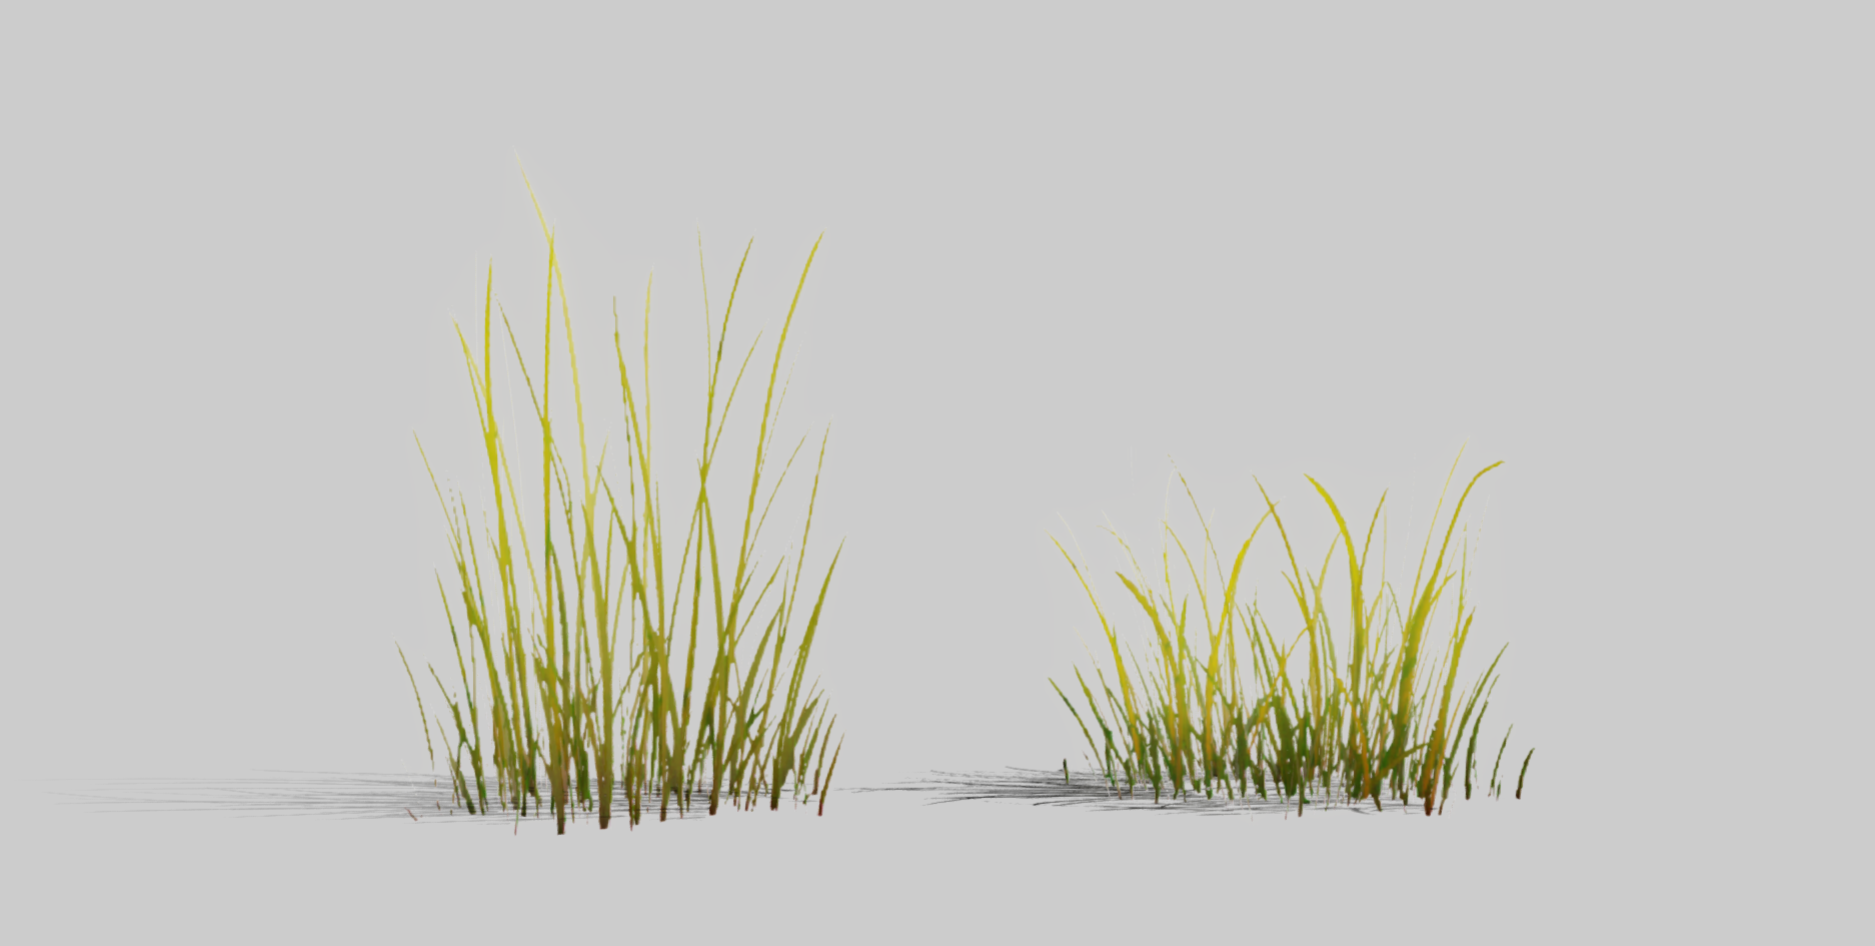
\includegraphics[width=\textwidth]{images/models/grass.png}
        \caption{Grass Model \cite{model-grass}} \label{fig:grass-model}
    \end{figure}
    \begin{figure}
        \centering
        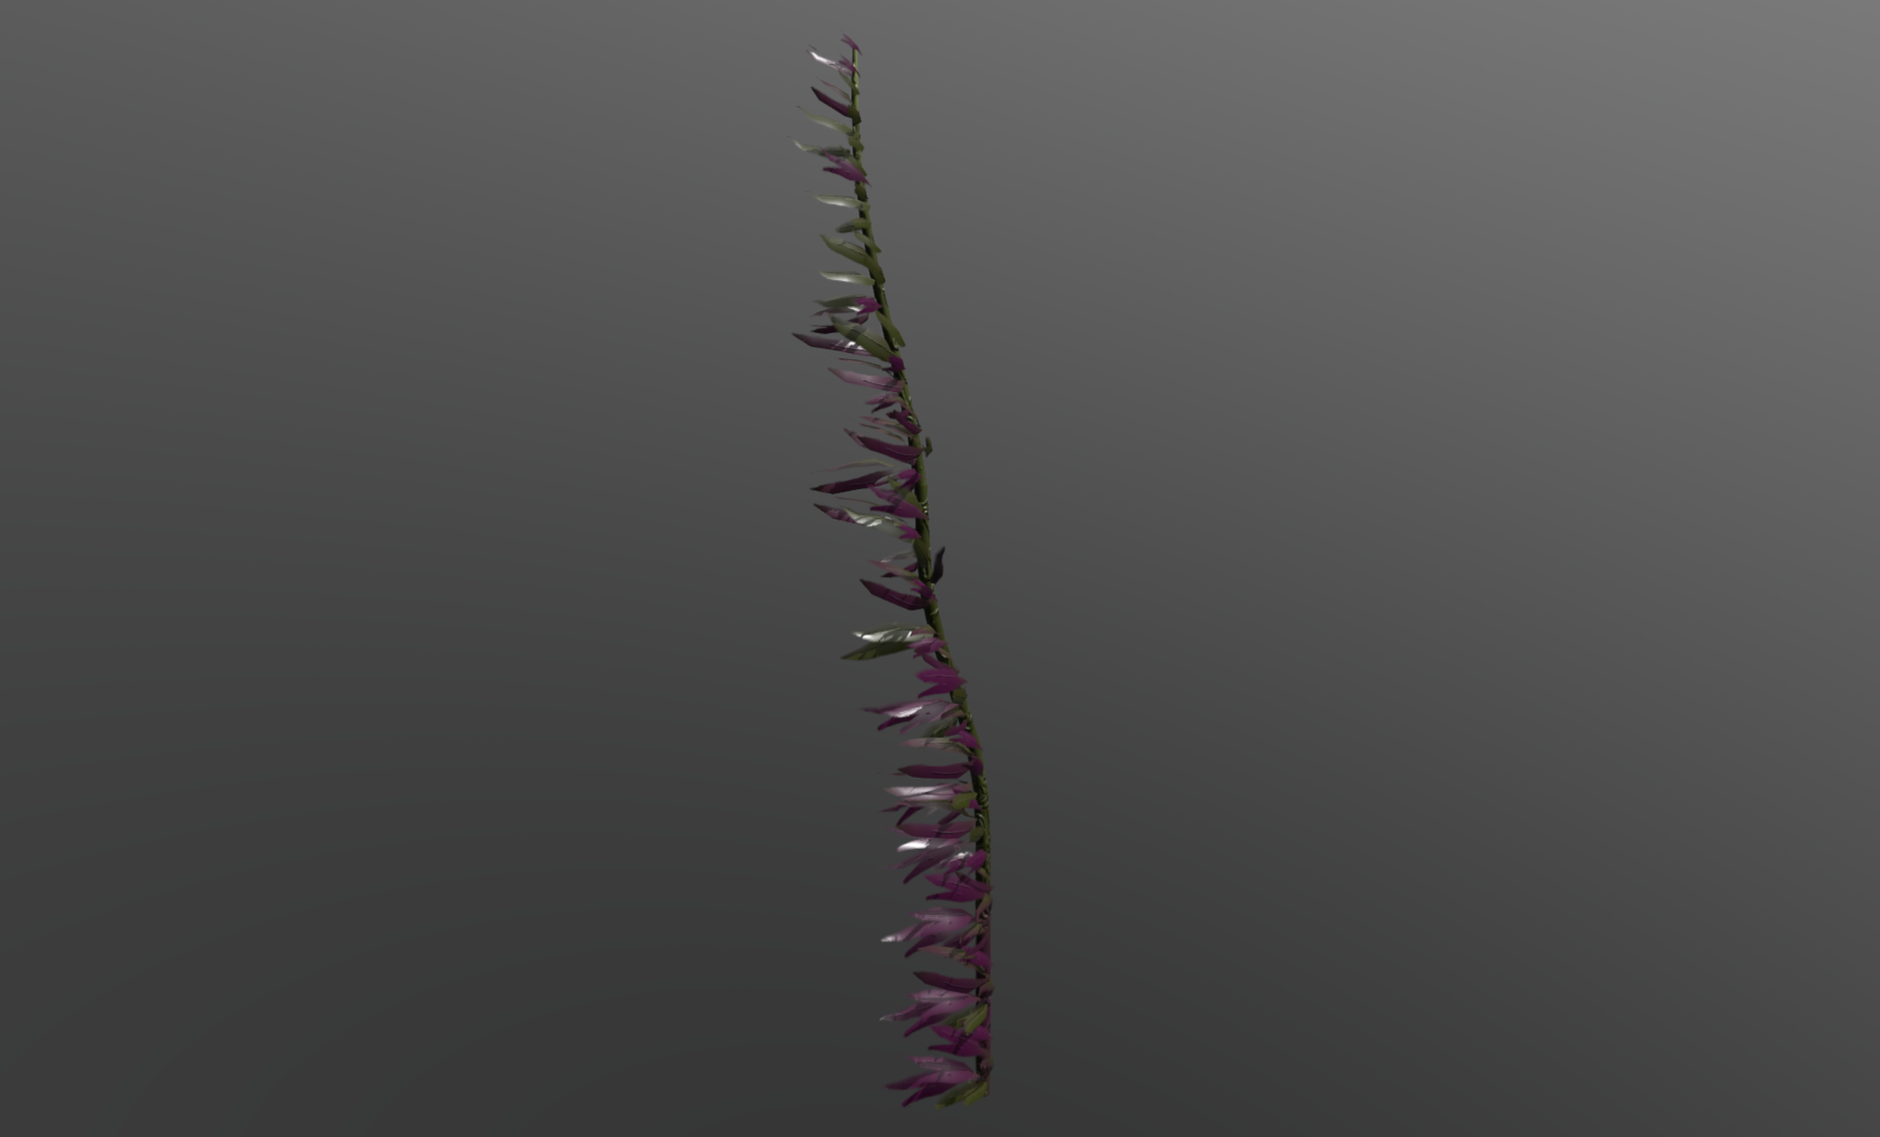
\includegraphics[width=\textwidth]{images/models/kelp.png}
        \caption{Kelp Model \cite{model-kelp}} \label{fig:kelp-model}
    \end{figure}
    \begin{figure}
        \centering
        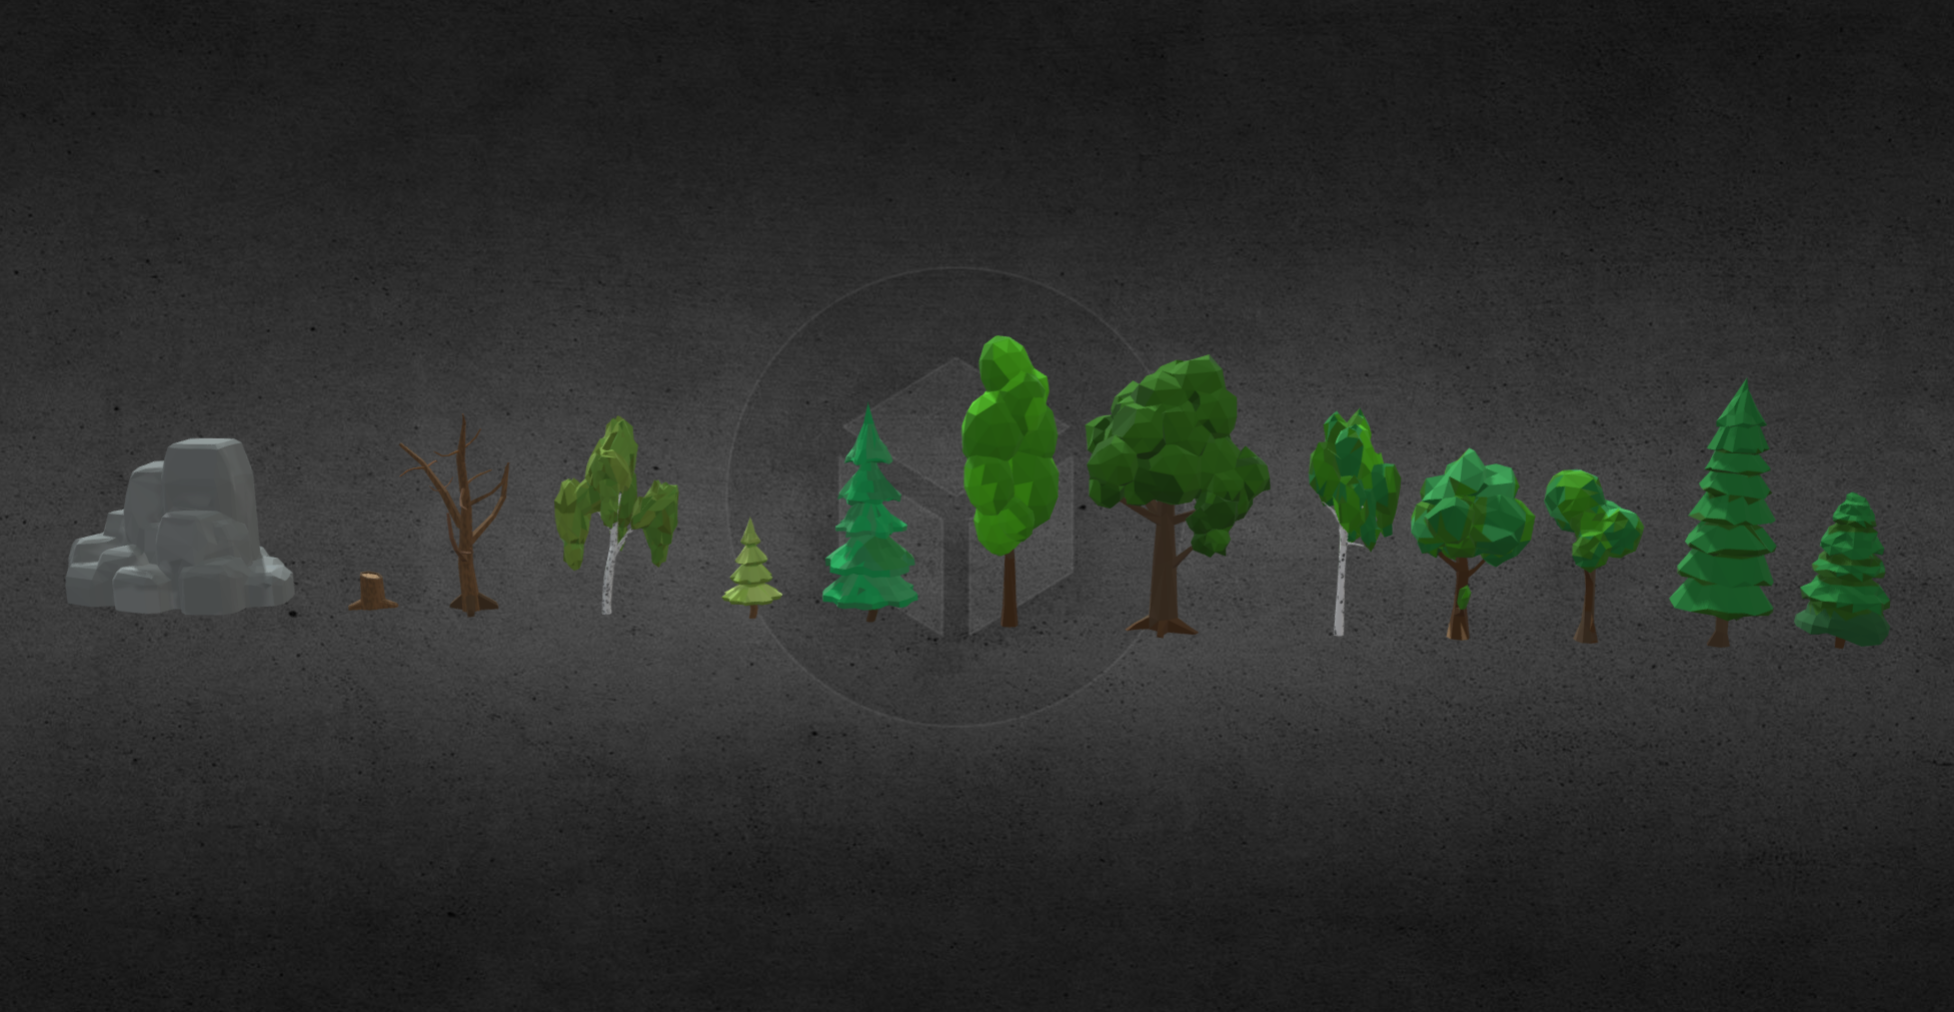
\includegraphics[width=\textwidth]{images/models/trees.png}
        \caption{Trres Model \cite{model-trees}} \label{fig:trees-model}
    \end{figure}
    \begin{figure}
        \centering
        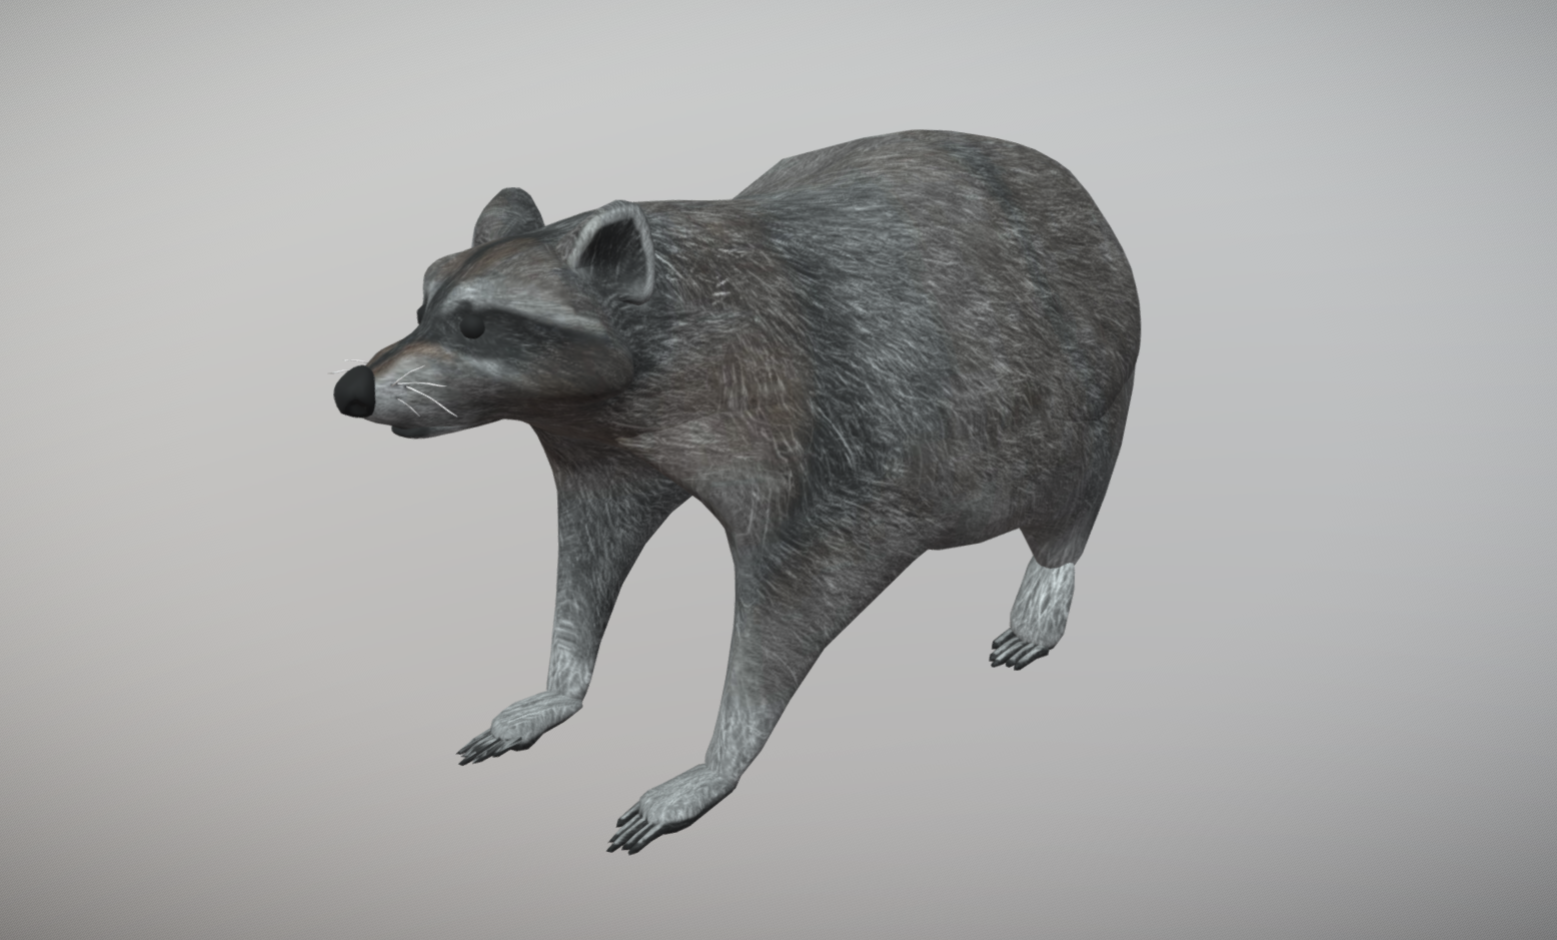
\includegraphics[width=\textwidth]{images/models/raccoon.png}
        \caption{Raccoon Model \cite{model-raccoon}} \label{fig:raccoon-model}
    \end{figure}
    \begin{figure}
        \centering
        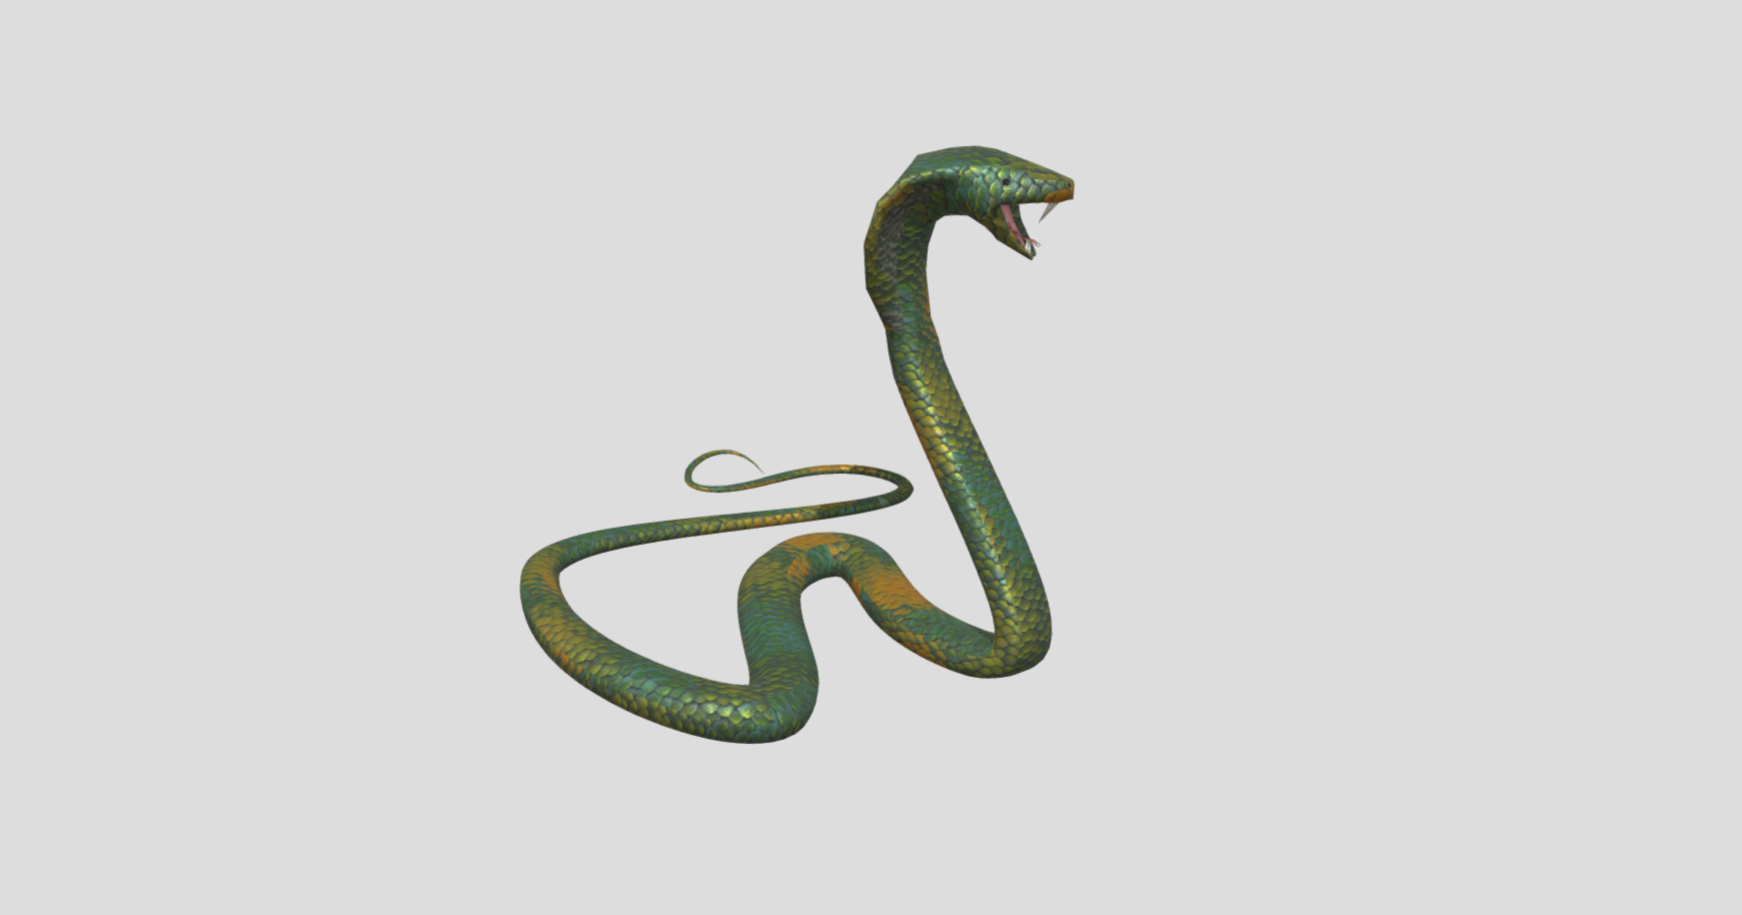
\includegraphics[width=\textwidth]{images/models/snake.png}
        \caption{Snake Model \cite{model-snake}} \label{fig:snake-model}
    \end{figure}
    \begin{figure}
        \centering
        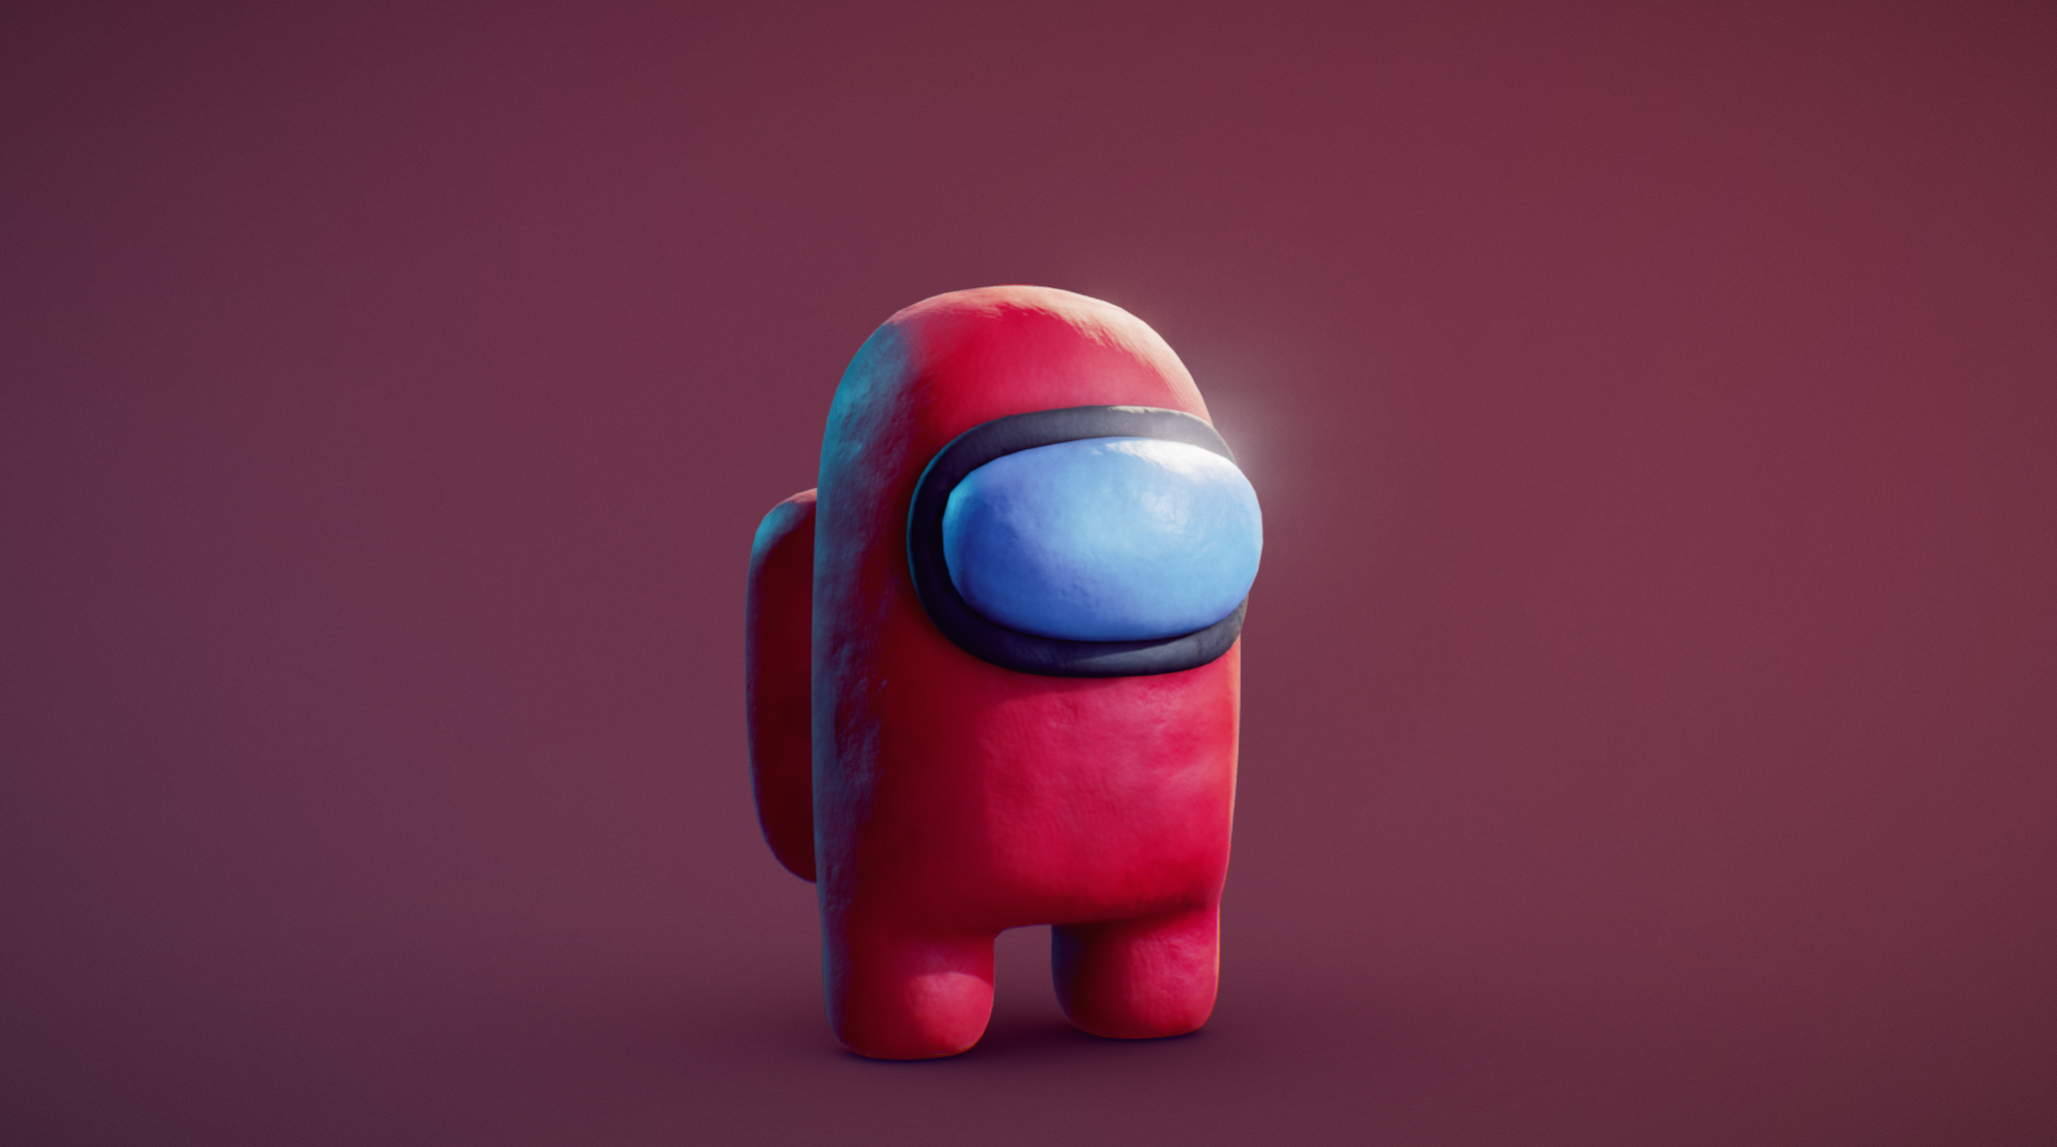
\includegraphics[width=\textwidth]{images/models/among_us.png}
        \caption{Among Us Model \cite{model-among-us}} \label{fig:among-us-model}
    \end{figure}
\end{document}
